\begingroup

\setcounter{chapter}{24}
\setcounter{chpnum}{24}

\fenicschapter{Improved Boussinesq equations for surface water waves}
              {Improved Boussinesq equations for surface \\ water waves}
              {Improved Boussinesq equations for surface water waves}
              {Nuno D. Lopes, Pedro J. S. Pereira and Lu{\'\i}s Trabucho}
              {lopes}

The main motivation of this work is the implementation of a general
finite element solver for some of the improved Boussinesq
models\index{Boussinesq model}. Here, we use an extension of the
model proposed by~\citet{ZhaoTengCheng2004} to investigate the
behavior of surface water waves. The equations in this model do not
contain spatial derivatives with an order higher than two. Some
effects like energy dissipation and wave generation by natural
phenomena or external physical mechanisms are also included. As a
consequence, some modified dispersion relations are derived for this
extended model. A matrix-based linear stability analysis of the
proposed model is presented. It is shown that this model is robust
with respect to instabilities related to steep bottom gradients.

\section{Overview}

The \fenics project, via \dolfin, \ufl and \ffc, provides good
technical and scientific support for the implementation of large scale
industrial models based on the finite element method. Specifically,
all the finite element matrices and vectors are automatically
generated and assembled by \dolfin\ and \ffc, directly from the
variational formulation of the problem which is declared using
\ufl. Moreover, \dolfin\ provides a user friendly interface for the
libraries needed to solve the finite element system of equations.

Numerical implementation of Boussinesq equations goes back to the
works of \citet{Peregrine1967} and \citet{Wu1981}, and later by the
development of improved dispersion characteristics (see, e.g.,
\citet{MadsenEtAl1991,Nwogu1993,ChenLiu1994} as well as
\citet{BejiNadaoka1996}).

We implement a solver for some of the Boussinesq type systems to model
the evolution of surface water waves\index{water waves} in a variable
depth seabed.  This type of model is used, for instance, in harbor
simulation (see Figure~\ref{fig:lopes:harbor} for an example of a
standard harbor), tsunami generation and wave propagation as well as
in coastal dynamics.

\begin{figure}[!t]
\centering
\includegraphics{0001335358/272415_1_en_25_fig1_print.tif}
\caption{Nazar\'{e}'s harbor, Portugal.}
\label{fig:lopes:harbor}\vspace*{6pt}
\end{figure}

In Section~\ref{sec:lopes:dolfwave}, we begin by describing the
DOLFWAVE application which is a \fenics based application for the
simulation of surface water waves (see
\url{https://launchpad.net/dolfwave}).

The governing equations for surface water waves are presented in
Section~\ref{sec:lopes:modelderivation}. From these equations
different types of models can be derived. There are several Boussinesq
models and some of the most widely used are those based on the wave
surface Elevation and horizontal Velocities formulation (BEV) (see,
e.g., \citet{WalkleyBerzins2002}, \citet{WooLiu2004a} as well as
\citet{WooLiu2004b} for finite element discretizations of BEV models).
However, we only consider the wave surface Elevation and velocity
Potential (BEP) formulation (see, e.g.,
~\citet{LangtangenPedersen1998}\vadjust{\pagebreak} for a finite element discretization of
a BEP model).  Thus, the number of unknowns is reduced from five (the
three velocity components, the pressure and the wave surface
elevation) in the BEV models to three (the velocity potential, the
pressure and the wave surface elevation) in the BEP models. Two
different types of BEP models are taken into account:
%%
\begin{enumerate}
\item \label{lopes:i}  a standard  model containing sixth-order
  spatial derivatives;
\item the  model proposed by~\citet{ZhaoTengCheng2004} (ZTC),
 containing only first and second-order spatial derivatives.
\end{enumerate}

A standard technique is used in order to derive the Boussinesq-type
model mentioned in~\ref{lopes:i}.  In the subsequent sections, only
the ZTC-type model is considered.  Note that these two models are
complemented with some extra terms, due to the inclusion of effects
like energy dissipation and wave generation by moving an impermeable
bottom or using a source function.

An important characteristic of the extended ZTC model, including
dissipative effects, is presented in
Section~\ref{sec:lopes:dispersionproperties}, namely, the dispersion
relation.


Section~\ref{sec:lopes:numericalmethods} is dedicated to the numerical
methods used in the discretization of the variational formulation.
The discretization of the spatial variables is accomplished with
Lagrange $P_1$ or $P_2$ finite elements (see
Chapter~\ref{chap:kirby-6}) whereas the time integration is
implemented using Runge--Kutta and predictor-corrector algorithms.

In Sections~\ref{sec:lopes:wavegeneration}
and~\ref{sec:lopes:boundaryconditions}, we describe several types of
wave generation, absorption and reflection mechanisms. Initial
conditions for a solitary wave and a periodic wave induced by
Dirichlet boundary conditions are also presented. Moreover, the
extended ZTC model includes a source function to generate surface
water waves, as proposed in \citet{WeiKirbySinha1999}. Total
reflective walls are modelled by standard zero Neumann conditions for
the wave surface elevation and velocity potential.  The wave energy
absorption is simulated using sponge layers.

\pagebreak

In Section~\ref{sec:lopes:linearanalysis}, we use a matrix-based
analysis in order to study some stability properties of the linearized
ZTC model in one horizontal dimension and with a time-independent
bathymetry. The standard potential model with depth averaged velocity
potential investigated by \citet{LovholtPedersen2009} is also used
here as a reference for comparison.

In Section~\ref{sec:lopes:numericaltests}, the extended ZTC equations
are used to model four different physical problems: the evolution of
solitary waves passing through submerged bars with different
geometries, the evolution of a Gaussian hump in a square basin, the
evolution of a periodic wave in a harbor geometry like that one
represented in Figure~\ref{fig:lopes:harbor} and the generation of a
wave due to an object moving on a horizontal bottom. We also use the
first numerical test to illustrate the usage of the DOLFWAVE
application.

Other solvers, mostly based on finite difference methods, have been
proposed in the literature, such like FUNWAVE (see \citet{Kirby1998}),
COULWAVE (see \citet{LynettLiu2004}) and the global Boussinesq solver
by \citet{PedersenLovholt2008}.  FUNWAVE is based on the fully
nonlinear and BEV equations by \citet{WeiKirby1995}.  Wave generation
by source function, wave breaking, bottom friction, treatment of
moving shorelines, subgrid turbulent mixing, totally reflective walls
and sponge layers are included in this model.  The third-order spatial
derivative equations in this model are discretized using a
fourth-order finite difference scheme.  Specifically, for time
integration, a composite fourth-order Adams--Bashforth--Moulton scheme
(third-order Adams--Bashforth predictor step and a fourth-order
Adams--Moulton corrector-step) is used.  Moreover, a fourth-order
Shapiro type filter is applied to remove short length waves.  The main
cause of instabilities in nonlinear shallow water computations is
often due to high nonlinearity in shallow water.  The instabilities
appear through fast growing short wavelengths which eventually cause
the blowup of the model.

COULWAVE possesses essentially the main features of FUNWAVE plus the
inclusion of wave generation due to a moving bottom.  Moreover,
COULWAVE is based on a multilayer third-order spatial derivative BEV
model.  This leads to improved dispersion relations and nonlinear
properties when compared with FUNWAVE.  However, the number of primary
unknowns in this two horizontal dimensional model with $n$-layers
increases from $3$ to $2n+1$. Thus, the computational time is also
increased, accordingly.

The global Boussinesq solver by \citet{PedersenLovholt2008} is based
on BEV and BEP models, although the BEV versions are preferred by the
authors.  In \citet{LovholtPedersen2009} several BEV and BEP models
are studied regarding linear stability properties.  It was shown that
the tested BEV formulations are less prone to instabilities due to
steep depth gradients than some BEP ones.  This solver includes
Coriolis effect and the modification on arc lengths by the curvature
of the Earth. The main goal of this solver is to treat, efficiently
and in a robust way, large scale ocean waves such as tsunamis.  The
shoreline runup, breaking waves or generation of waves by moving
bottoms are not yet included.  Only standard nonlinear terms are
considered and finite differences methods are used to discretize the
model, specifically C-grid is implemented for the spatial
discretization and a leap-frog scheme is used for the time stepping.

\vspace*{5pt}
\section{DOLFWAVE}
\label{sec:lopes:dolfwave}

The main goal of DOLFWAVE is to provide a framework for the analysis,
development and computation of models for surface water waves, based
on finite element methods. Algorithms for shoreline runup/rundown,
numerical filters or effects like wave breaking or bottom friction are
not yet included in the application, however they are planned for
future implementation.

\pagebreak

We have already implemented solvers for the following cases:
\begin{enumerate}
\item \label{lopes:list_i} Shallow water wave models for
  unidirectional long waves in one horizontal dimension;
\item  Boussinesq-type models for moderately long
  waves with small amplitude in shallow water.
\end{enumerate}
%%
The shallow water wave models implemented and mentioned in
\ref{lopes:list_i} are the following:
\begin{itemize}
\item The Korteweg--de Vries (KdV) model which consists of a weakly
  nonlinear and dispersive third-order partial differential equation
  for the wave surface elevation. The discretization of the spatial
  variable is accomplished using a continuous/discontinuous finite
  element method with Lagrange $P_2$ elements;
\item The Benjamin--Bona--Mahony model, also known as the regularized
  long-wave (RLW) model, which is an improvement of the KdV model
  regarding the dispersive properties.  The equation in the RLW model
  contains only second-order spatial derivatives. The discretization
  of the spatial variable is accomplished using continuous finite
  element methods with Lagrange $P_1$ or $P_2$ elements.
\end{itemize}
%%
For the Boussinesq-type models we considered the following
cases:
%%
\begin{itemize}
\item The extended ZTC model which is based on a system of two
  second-order partial differential equations for the wave surface
  elevation and a velocity potential. The discretization of the
  spatial variables is accomplished using continuous finite element
  methods with Lagrange $P_1$ or $P_2$ elements;
 \item An extension of the model by \citet{ChenLiu1994} in order to
   include dissipative effects, several forms of wave generation and
   improved dispersive properties. This model is based on a system of
   two fourth-order partial differential equations for the wave
   surface elevation and a velocity potential. The discretization of
   the spatial variables is accomplished using the
   continuous/discontinuous finite element method with Lagrange $P_2$
   elements (see~\citet{LopesPereiraTrabucho}).
\end{itemize}

A predictor-corrector scheme with an initialization provided by an
explicit Runge--Kutta method is used for the time integration of the
equations.  These schemes are easier to implement and require smaller
computational times than the implicit ones.  However, they are more
prone to numerical instabilities and in general require smaller time
steps.

We use \ufl\ for the declaration of the finite element discretization
of the variational forms related to the models mentioned above (see
the \ufl\ form files in the following directories of the DOLFWAVE code
tree: \emp{dolfwave/src/1hd1sforms}, \emp{dolfwave/src/1hdforms} and
\emp{dolfwave/src/2hdforms}).  These files are compiled using \ffc to
generate the C++ code of the finite element discretization of the
variational forms (see Chapter~\ref{chap:alnes-1}).  DOLFWAVE is based
on the C++ interface of DOLFIN $1.0$ to assemble and solve all the
systems of equations related with the finite element method.

All the DOLFWAVE code is available for download at
\url{https://launchpad.net/dolfwave}. Some tools for the generation of
the C++ code for boundary conditions and source functions are
included. Scripts for visualization and data analysis are also part of
the application. The Xd3d post-processor is used in some cases (see
\url{http://www.cmap.polytechnique.fr/~jouve/xd3d/}).  DOLFWAVE has a
large number of demos covering all the implemented models (see
\emp{dolfwave/demo}). Different physical effects are illustrated.  All
the numerical examples in this work are included in the demos.

\pagebreak

\section{Model derivation}
\label{sec:lopes:modelderivation}

We consider the following set of equations for the irrotational flow
of an incompressible and inviscid fluid:

\begin{subequations}\label{eq:lopes:euler}
\begin{align}
&\displaystyle\frac{\partial u}{\partial t}+ u \cdot \nabla
  u=-\nabla\left(\frac{P}{\rho} +g\,
  z\right),\label{eq:lopes:euler-a} \\[2pt] &\nabla\times
  u={0},\label{eq:lopes:euler-b}\\[2pt]
  &\nabla\cdot{u}=0,\label{eq:lopes:euler-c}
\end{align}
\end{subequations}
%%
where $u$ is the velocity vector field of the fluid, $P$ the pressure,
$g$ the gravitational acceleration, $\rho$~the mass per unit volume,
$t$ the time and the differential operator
$\nabla=\left(\frac{\partial }{\partial x},\frac{\partial }{\partial
y},\frac{\partial }{\partial z}\right).$ A Cartesian coordinate system
is adopted with the horizontal $x$ and $y$-axes on the still water
plane and the $z$-axis pointing vertically upwards (see
Figure~\ref{fig:lopes:schematic}).  The fluid domain is bounded by the
bottom seabed at $z=-h(x,y,t)$ and the free water surface at
$z=\eta(x,y,t)$.  In Figure~\ref{fig:lopes:schematic}, $L$, $A$ and
$H$ are the characteristic wave length, wave amplitude and depth,
respectively. Note that the material time derivative is denoted by
$\frac{D}{D t}$.

\begin{figure}[!b]
%\bwfig
\centering
%\fenicsfig{lopes}{graph}{\largefig}
%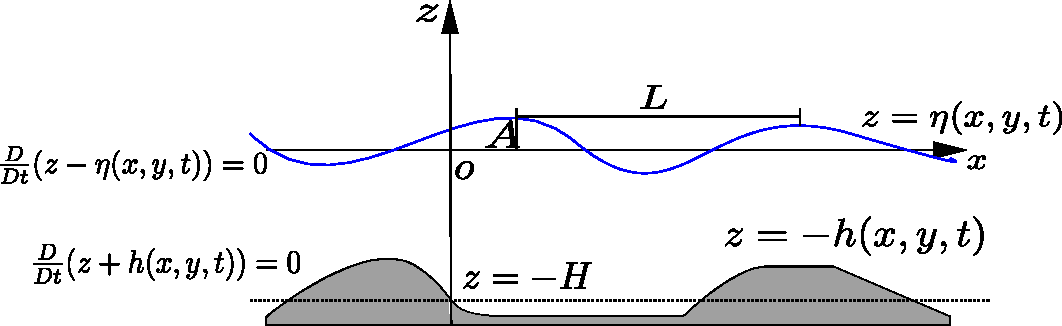
\includegraphics[width=\largefig]{lopes/graph}
\includegraphics{0001335358/272415_1_en_25_fig2_print.eps}
\caption{Cross-section of the water wave domain.}
\label{fig:lopes:schematic}
\end{figure}

From the irrotational assumption (see ~\eqref{eq:lopes:euler-b}), we
can introduce a velocity potential function,
$\phi(x,y,z,t)$\index{potential} to obtain Bernoulli's equation:\vspace*{-3pt}
\begin{equation}
\label{eq:lopes:bern}
\frac{\partial \phi}{\partial t}+\frac{1}{2}\nabla \phi \cdot\nabla
\phi + \frac{P}{\rho} +g\, z=f(t),\vspace*{-3pt}
\end{equation}
%%
where $u=\nabla\phi(x,y,z,t)$ and $f(t)$ stands for an arbitrary
function of integration.  Note that we can remove $f(t)$ from
equation~\eqref{eq:lopes:bern} if $\phi$ is redefined by $\phi+\int
f(t) \dt$.  From the incompressibility condition
(see~\eqref{eq:lopes:euler-c}) the velocity potential satisfies
Laplace's equation:\vspace*{-3pt}
\begin{equation}
  \label{eq:lopes:lap}
  \nabla^2\phi+\frac{\partial^2\phi}{\partial z^2}=0,\vspace*{-3pt}
\end{equation}
%%
where, from now on, $\nabla$ denotes the horizontal gradient operator
given by $\nabla=\left(\frac{\partial }{\partial
    x},\frac{\partial}{\partial y}\right)\!\!.$ To close this problem,
the following boundary conditions must be satisfied:

\begin{enumerate}
\item the kinematic boundary condition for the free water
  surface:\vspace*{-3pt}
  \begin{equation}
    \frac{\partial \phi}{\partial
      z}=\frac{\partial\eta}{\partial
      t}+\nabla\phi\cdot\nabla\eta,\quad z=\eta;\vspace*{-3pt}
  \end{equation}
\item the kinematic boundary condition for the
  impermeable sea bottom:\vspace*{-3pt}
  \begin{equation}
    \frac{\partial \phi}{\partial z}+(\nabla\phi\cdot\nabla
    h)=-\frac{\partial h}{\partial t}, \quad z=-h;\vspace*{-3pt}
  \end{equation}
\item the dynamic boundary condition for the
  free water surface:\vspace*{-3pt}
  \begin{equation}\label{eq:lopes:dyn}
    \frac{\partial \phi}{\partial t}+ g\eta+\frac{1}{2}
    \left(|\nabla\phi|^2 + \left(\frac{\partial \phi}{\partial
          z}\right)^2\right)+ D(\phi) = 0, \quad z =\eta,\vspace*{-3pt}
  \end{equation}
\end{enumerate}
%%
where $D(\phi)$ is a dissipative term (see, e.g., the work
by~\citet{DutykhDias2007}).  We assume that this dissipative term is
of the following form:\vspace*{-2pt}
%%
\begin{equation}
  \label{eq:lopes:diss}
  D(\phi)=\nu\frac{\partial ^2\phi}{\partial z^2},
\end{equation}
%%
with $\nu=\bar{\mu}/\rho$ and $\bar{\mu}$ an eddy-viscosity
coefficient.  Note that a non-dissipative model means that there is no
energy loss.  This is not acceptable from a physical point of view,
since any real flow is accompanied by energy dissipation.

Using Laplace's equation (see~\eqref{eq:lopes:lap}) it is possible to
rewrite~\eqref{eq:lopes:diss} as $D(\phi)=-\nu\nabla^2\phi$.
Throughout the literature, analogous terms were added to the kinematic
and dynamic conditions to absorb the wave energy near the boundaries.
These terms are related with the sponge or damping layers and, as we
will see later, they can be used to modify the dispersion relations.

A more detailed description of the above equations is found in the
reference book on waves by~\citet{Whitham1974}, or in the more recent
book by~\citet{Johnson1997}.

\subsection{Standard models}

In this subsection, we present a generic Boussinesq system using the
velocity potential formulation.  To transform
equations~\eqref{eq:lopes:bern}--~\eqref{eq:lopes:diss} in a
dimensionless form, the following scales are introduced (see
Figure~\ref{fig:lopes:schematic}):
%%
\begin{equation}
( x', y')=\frac{1}{L}(x,y),\quad z'=\frac{z}{H}, \quad
t'=\frac{t\sqrt{gH}}{L},\quad \eta'=\frac{\eta}{A},\quad
\phi'= \frac{H\phi}{AL\sqrt{gH}},\quad h'=\frac{h}{H},
\end{equation}
%%
together with the small parameters
%%
\begin{align}
  \mu=\frac{H}{L},\quad \varepsilon=\frac{A}{H}.
\end{align}
%%
In the last equation, $\mu$ is called the long wave parameter and
$\varepsilon$ the small amplitude wave parameter.  Note that
$\varepsilon$ is related with the nonlinear terms and $\mu$ with the
dispersive terms.  For simplicity, in what follows, we drop the prime
notation.

The Boussinesq approach consists of reducing a $3$D problem to a $2$D
one.  This may be accomplished by expanding the velocity potential in
a Taylor power series in terms of $z$.  Using Laplace's equation, in a
dimensionless form, we can obtain the following expression for the
velocity potential:
%%
\begin{equation}
\phi(x,y,z,t) = \sum_{n=0}^{+\infty} \left((-1)^n \frac{z^{2n}}{(2n)!}
  \mu^{2n}\nabla^{2n}\phi_0(x,y,t) + (-1)^n \frac{z^{2n+1}}{(2n+1)!}
  \mu^{2n}\nabla^{2n}\phi_1(x,y,t)\right),
\end{equation}
%%
with
%%
\begin{align}
  \phi_0=\phi\mid_{ z=0},\quad
  \phi_1=\left(\frac{\partial \phi}{\partial z}\right)\mid_{z=0}\!.
\end{align}
%%
From asymptotic expansions, successive approximation techniques and
the kinematic boundary condition for the sea bottom, it is possible to
write $\phi_1$ in terms of $\phi_0$ (see~\citet{ChenLiu1994}
and~\citet{ZhaoTengCheng2004}).  In this work, without loss of
generality, we assume that the dispersive and nonlinear terms are
related by the following equation:
%%
\begin{equation}
  \label{eq:lopes:ursell}
  \frac{\varepsilon}{\mu^2}=O(1)\ {\rm with}\ \mu<1\ {\rm
    and}\ \varepsilon<1.
\end{equation}
%%
Note that the Ursell number is defined by $U_r = \varepsilon/\mu^2$
and plays a central role in deciding the choice of approximations
which correspond to very different physics.  The regime of weakly
nonlinear, small amplitude and moderately long waves in shallow water
is characterized by \eqref{eq:lopes:ursell}
$\left(O(\mu^2)=O(\varepsilon)\right.$; that is,
$\left.\frac{H^2}{L^2}\sim\frac{A}{H} \right)$. Boussinesq equations
account for the effects of nonlinearity $\varepsilon$ and dispersion
$\mu^2$ to the leading order.  When $\varepsilon\gg \mu^2$ , they
reduce to the Airy equations.  When $\varepsilon\ll \mu^2$ they reduce
to the linearized approximation with weak dispersion.  Finally, if we
assume that $\varepsilon\rightarrow 0$ and $\mu^2\rightarrow 0$, the
classical linearized wave equation is obtained.

A sixth-order spatial derivative model is obtained if $\phi_1$ is
expanded in terms of $\phi_0$ and all terms up to $O(\mu^8)$ are
retained.  Thus, the asymptotic kinematic and dynamic boundary
conditions for the free water surface are rewritten as follows
\footnote{Note that $D$ is, now, a dimensionless function.}:
%%
\begin{subequations}
  \label{eq:lopes:kindyn}
  \begin{align}
    &\displaystyle\frac{\partial \eta}{\partial
      t}+\varepsilon\nabla\cdot(\eta\nabla\phi_0) -
    \frac{1}{\mu^2}\phi_1 +
    \frac{\varepsilon^2}{2}\nabla\cdot(\eta^2\nabla\phi_1)=O(\mu^{6}),
    \\[2pt] &\displaystyle
    \frac{\partial \phi_0}{\partial t}+\varepsilon\eta\frac{\partial
      \phi_1}{\partial t}+\eta + \frac{\varepsilon}{2}
    \left|\nabla\phi_0\right|^2 +
    \varepsilon^2\nabla\phi_0\cdot\eta\nabla\phi_1\nonumber
    \\[2pt] & \displaystyle \qquad
    -\varepsilon^2\eta\nabla^2\phi_0\phi_1
    +\frac{\varepsilon}{2\mu^2}\phi_1^2
    +D(\phi_0,\phi_1)
    =O(\mu^{6}),
  \end{align}
\end{subequations}
%%
where $\phi_1$ is given by:
%%
\begin{multline}\label{eq:lopes:phi_1}
  \phi_1= -\mu^{2}\nabla\cdot\left(h\nabla\phi_0\right)
  +\frac{\mu^{4}}{6}\nabla\cdot\left(h^3\nabla^3\phi_0\right)
  -\frac{\mu^{4}}{2}\nabla\cdot\left(h^2
    \nabla^2\cdot\left(h\nabla\phi_0\right) \right)\\[2pt]
  -\frac{\mu^6}{120}\nabla\cdot\left(h^5\nabla^5\phi_0\right)+
  \frac{\mu^6}{24}\nabla\cdot\left(h^4\nabla^4\cdot
    \left(h\nabla\phi_0\right)\right) +
  \frac{\mu^6}{12}\nabla\cdot\left(h^2\nabla^2\cdot
    \left(h^3\nabla^3\phi_0\right)\right)\\[2pt]
  - \frac{\mu^6}{4}\nabla\cdot\left(h^2\nabla^2 \cdot
    \left(h^2\nabla^2\cdot\left(h\nabla\phi_0\right)\right)\right)
  -\frac{\mu^2}{\varepsilon}\frac{\partial h}{\partial t}-
  \frac{\mu^2}{\varepsilon}\frac{\mu^2}{2}\nabla \cdot
  \left(h^2\nabla\frac{\partial - h}{\partial t}\right)\\[2pt]
  +\frac{\mu^2}{\varepsilon}\frac{\mu^4}{24}\nabla \cdot
  \left(h^4\nabla^3 \frac{\partial h}{\partial t}\right)
  -\frac{\mu^2}{\varepsilon}\frac{\mu^4}{4}\nabla \cdot
  \left(h^2\nabla^2\left(h^2\nabla\frac{\partial h}{\partial
        t}\right)\right)+O(\mu^{8}).
\end{multline}
To obtain equation~\eqref{eq:lopes:phi_1}, we assume that
$\displaystyle\frac{\partial h}{\partial t}=O(\varepsilon)$
(see~\citet{DutykhDias2007}).

\subsection{Second-order spatial derivative model}
The second-order spatial derivative equations are obtained,
essentially, via the slowly varying bottom assumption. In particular,
only $O(h,\nabla h)$ terms are retained.  Also, only $O(\varepsilon)$
nonlinear terms are admitted.  In fact, the extended ZTC model is
written retaining only $O(\varepsilon,\mu^4)$ terms.

\pagebreak

Under these conditions, \eqref{eq:lopes:kindyn} and~\eqref{eq:lopes:phi_1}
lead to:
%%
\begin{subequations}
\label{eq:lopes:kindyn2}
\begin{align} &\displaystyle\frac{\partial \eta}{\partial
    t}+\varepsilon\nabla\cdot(\eta\nabla\phi_0)
  -\frac{1}{\mu^2}\phi_1=O(\mu^{6}),
  \label{eq:lopes:kindyn2-a}
  \\[2pt] &\displaystyle\frac{\partial \phi_0}{\partial t}+\eta +
  \frac{\varepsilon}{2}
  \left|\nabla\phi_0\right|^2-\nu^*\varepsilon\nabla^2\phi_0
  =O(\mu^{6}),
  \label{eq:lopes:kindyn2-b}
\end{align}
\end{subequations}
%%
where $\nu^*=\nu\sqrt{H}/(AL\sqrt{g})$ and
%%
\begin{multline}
\label{eq:lopes:phi_2}
\phi_1= -\mu^{2}\nabla\cdot\left(h\nabla\phi_0\right)
+\frac{\mu^{4}}{6}\nabla\cdot\left(h^3\nabla^3\phi_0\right)
-\frac{\mu^{4}}{2}\nabla\cdot\left(h^2
\nabla^2\cdot\left(h\nabla\phi_0\right)
\right)\\[2pt]
-\frac{2\mu^6}{15}h^5\nabla^6\phi_0-2\mu^6h^4\nabla
h\cdot\nabla^5\phi_0
-\frac{\mu^2}{\varepsilon}\frac{\partial h}{\partial t}+O(\mu^{8}).
\end{multline}
%%
Thus, these extended equations are written as follows:
%%
\begin{subequations}
\label{eq:lopes:ztcdimensionless}
\begin{align}
  &\frac{\partial\eta}{\partial t}
  +\nabla\cdot[(h+\varepsilon\eta)\nabla{\Phi}] -\frac{\mu^2}{2}
  \nabla\cdot \left[h^{2}\nabla\frac{\partial \eta} {\partial t}\right]
  +\frac{\mu^2}{6}h^{2}\nabla^2\frac{\partial\eta}{\partial t}
  -\frac{\mu^2}{15}\nabla\cdot\left[h\nabla\left(h\frac{\partial\eta}
  {\partial t}\right)\right]=-\frac{1} {\varepsilon}\frac{\partial h}{\partial
    t}, \label{eq:lopes:ztcdimensionless-a}\\ &\frac{\partial
    \Phi}{\partial t} +\frac{\varepsilon}{2}|\nabla\Phi|^2+\eta-
  \frac{\mu^2}{15}h\nabla\cdot(h\nabla\eta)-\nu^*\varepsilon
  \nabla^2\Phi = 0,
  \label{eq:lopes:ztcdimensionless-b}
\end{align}
\end{subequations}
%%
where $\Phi$ is the transformed velocity potential given by:
%%
\begin{equation}
  \label{eq:lopes:phitransdimensionless}
  \Phi=\phi_0+\mu^2\frac{h}{15}\nabla\cdot(h\nabla\phi_0).
\end{equation}
%%
In terms of the dimensional variables,
equations~\eqref{eq:lopes:ztcdimensionless} become:
%%
\begin{subequations}
  \label{eq:lopes:ztc}
  \begin{align}
    &\frac{\partial\eta}{\partial t}
    +\nabla\cdot[(h+\eta)\nabla{\Phi}] -\frac{1}{2}\nabla\cdot
    \left[h^{2}\nabla\frac{\partial \eta} {\partial t}\right]
    +\frac{1}{6}h^{2}\nabla^2\frac{\partial\eta}{\partial t}
    -\frac{1}{15}\nabla\cdot\left[h\nabla\left(h\frac{\partial\eta}
    {\partial t}\right)\right] = -\frac{\partial h}{\partial t},
    \label{eq:lopes:ztc-a}\\ &\frac{\partial\Phi} {\partial t}
    +\frac{1}{2}|\nabla\Phi|^2+g\eta- \frac{1}{15}gh\nabla \cdot
    (h\nabla\eta)-\nu\nabla^2\Phi=0,
    \label{eq:lopes:ztc-b}
  \end{align}
\end{subequations}
%%
whereas equation~\eqref{eq:lopes:phitransdimensionless} is rewritten
as follows:
%%
\begin{equation}
  \label{eq:lopes:phitrans}
  \Phi=\phi_0+\frac{h}{15}\nabla\cdot(h\nabla\phi_0).
\end{equation}
%%
In this context, the use of the transformed velocity potential has two
main advantages (see~\citet{ZhaoTengCheng2004}):
%%
\begin{enumerate}
\item the spatial derivative order is reduced to 2;
\item linear dispersion characteristics, analogous to the
  BEP model proposed by \citet{ChenLiu1994} and the  BEV model
  developed by \citet{Nwogu1993}, are obtained. The latter models
  contain fourth and third-order spatial derivatives, respectively.
\end{enumerate}

\section{Linear dispersion relation}
\label{sec:lopes:dispersionproperties}

One of the most important properties of a water wave model is
described by the linear dispersion relation.  From this relation we
can deduce the phase velocity, group velocity and the linear shoaling.

The dispersion relation \index{dispersion relation} of a linearized
water wave model should be in good agreement with the one provided by
the linear wave theory of Airy.

In this section, we follow the work by~\citet{DutykhDias2007}.
Moreover, we only present a generalized version of the dispersion
relation for the extended ZTC model with the dissipative term
mentioned above.  We can also include other damping terms, which are
usually used in the sponge layers.

For simplicity, a one horizontal dimensional model is considered.  To
obtain the dispersion relation, a standard test wave is assumed:
%%
\begin{subequations}
  \label{eq:lopes:linwave}
  \begin{align}
    &\eta(x,t)=a\,e^{i(kx-\omega
      t)},\\
    &\Phi(x,t)=-b\,i\,e^{i(kx-\omega t)},
  \end{align}
\end{subequations}
%%
where $a$ is the wave amplitude, $b$ the potential magnitude,
$k=2\pi/L$ the wave number and $\omega$ the angular frequency.  This
wave, described by equations~\eqref{eq:lopes:linwave}, is the solution
of the linearized extended ZTC model, with a constant depth bottom and
an extra dissipative term, if the following equation is satisfied:
%%
\begin{equation}
  \label{eq:lopes:dissdisp}
  \omega^2-ghk^2\frac{1+\frac{1}{15}(kh)^2}{1 +
  \frac{2}{5}(kh)^2} + i\nu\omega k^2=0.
\end{equation}
%%
The dispersion relation given by the last equation is accurate up to
$O((kh)^4)$ or $O(\mu^4)$ when compared with the Pad\'{e} approximant
of order $[2/2]$ of the following equation:
%%
\begin{equation}
  \label{eq:lopes:linairy}
  \omega^2-ghk^2\frac{\tanh(kh)}{kh} + i\nu\omega k^2 = 0.
\end{equation}
%%
In fact, equation~\eqref{eq:lopes:linairy} is the dispersion relation
of the full linear problem.
%%

From~\eqref{eq:lopes:dissdisp}, the phase velocity, $C= w/k$, for this
dissipative and extended ZTC model is given~by:
%%
\begin{equation}
\label{eq:lopes:phasevel}
C = -\frac{i\nu k}{2}\pm\sqrt{-\left(\frac{\nu
      k}{2}\right)^2+gh\frac{(1+\frac{1}{15}(kh)^2)}{(1+\frac{2}{5}(kh)^2)}}.
\end{equation}
%%
In Figure~\ref{fig:lopes:dispersion}, we can see the positive real
part of $\displaystyle\left(C/\sqrt{gh}\right)$ as a function of $kh$
for the following models: full linear theory (FL), Zhao et al. (ZTC),
full linear theory with a dissipative model (FL\_D) and the improved
ZTC model with the dissipative term (ZTC\_D).
%%
\begin{figure}
  \centering
  %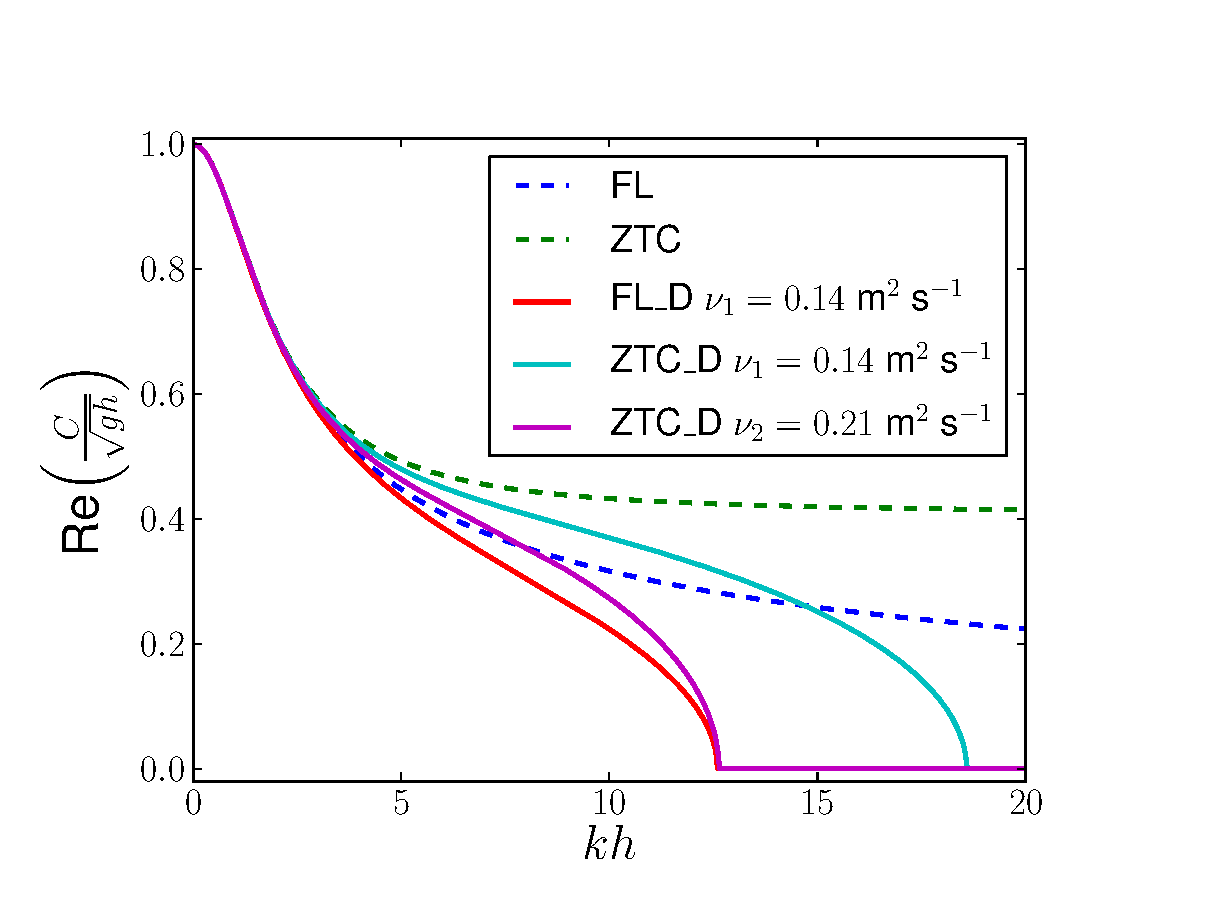
\includegraphics[width=\largefig]{chapters/lopes/pdf/phase_velocity_simple.pdf}
  \includegraphics{0001335358/272415_1_en_25_fig3_print.eps}
  \caption{Positive part of $\displaystyle
    Re\left(C/\sqrt{gh}\right)$ as a function of $kh$ for
    several models.}
  \label{fig:lopes:dispersion}
\end{figure}

From Figure~\ref{fig:lopes:dispersion}, we can also see that
these two dissipative models admit critical wave numbers $k_1$ and
$k_2$, such that the positive part of $\displaystyle
Re\left(C/\sqrt{gh}\right)$ is zero for $k\geqslant k_1$ and
$k\geqslant k_2$, respectively.  We can optimize the value of $\nu$ in
the ZTC\_D model in order to have $k_1=k_2$.  From
\eqref{eq:lopes:linairy}, $\displaystyle Re\left(C/\sqrt{gh}\right)$
is zero for
%%
\begin{equation}
  k_1^3=4g\frac{\tanh{(k_1h)}}{\nu^2}.
\end{equation}
%%
Thus, we can obtain the values of $k_1$, in the FL\_D model, for which
short waves no longer propagate for fixed $h$ and $\nu=\nu_1$ values.
Considering now the real part of \eqref{eq:lopes:phasevel} equal to
zero, we have
%%
\begin{equation}
\label{eq:lopes:nu1}
\nu^2=4\frac{gh}{k^2}\left(\frac{1+\frac{1}{15}(kh)^2}{1 +
    \frac{2}{5}(kh)^2}\right).
\end{equation}
%%
\looseness1{}Therefore, inserting the previous value of $k_1$ into
\eqref{eq:lopes:nu1} we obtain the corresponding value of $\nu=\nu_2$,
in the ZTC\_D model, for which the same type of waves do not
propagate.  As in~\citet{DutykhDias2007} we choose $\nu_1=0.14$\,{\tt
m$^2$\,s$^{-1}$}.  In Figure~\ref{fig:lopes:dispersion}, we can see
that if $\nu_1=0.14\,$~{\tt m$^2\,$s$^{-1}$} in the FL\_D model and
$\nu_2=0.21\,$~{\tt m$^2$\,s$^{-1}$} in the ZTC\_D model,
$k_1=k_2=12.6$\,{\tt m$^{-1}$} for $h=1$\,{\tt m}.  In this case the
time decay of the solutions in the ZTC\_D model is more accentuated
than in the FL\_D model.  Some instabilities generated by short length
waves can be eliminated optimizing the viscosity values as shown
above.

In general, to improve the dispersion relation we can also use other
transformations like~\eqref{eq:lopes:phitrans}, or evaluate the
velocity potential at $z=-\sigma h$ ($\sigma\in[0,1]$) instead of
$z=0$ (see~\citet{BinghamMadsenFuhrman2008}, \citet{MadsenAgnon2003}
and~\citet{MadsenBinghamSchaffer2003}).

%\enlargethispage{10pt}

\section{Numerical methods}
\label{sec:lopes:numericalmethods}
We start this section by noting that a detailed description of the
implemented numerical methods referred bellow can be found in the work
of \citet{Lopes2007}.

For simplicity, we only consider the system described by
equations~\eqref{eq:lopes:ztc} restricted to a stationary bottom and
without dissipative or extra source terms.

The model variational formulation is written as follows:
%%
\begin{subequations}
  \label{eq:lopes:varform}
  \begin{align}
    \begin{split}
      &\displaystyle \int_\Omega\frac{\partial \eta}{\partial
        t}\vartheta_1\, \dx\, \mathrm{d}y +\frac{1}{2}\int_\Omega
      h^2\nabla\left(\frac{\partial \eta}{\partial t}\right)
      \cdot\nabla\vartheta_1\, \dx\, \mathrm{d}y-
      \frac{1}{6}\int_\Omega \nabla\left(\frac{\partial \eta}{\partial
          t}\right)\cdot\nabla(h^2\vartheta_1)\, \dx\, \mathrm{d}y\\[2pt]
      &\quad \quad\displaystyle +
      \frac{1}{15}\int_\Omega
      h\nabla\left(h\frac{\partial \eta}{\partial t}\right)\cdot
      \nabla\vartheta_1\, \dx\, \mathrm{d}y- \frac{1}{15}\int_\Gamma
      h\frac{\partial h}{\partial n}\,\frac{\partial \eta}{\partial
        t}\,\vartheta_1\, \ds
      \\[2pt] &\quad\quad=\displaystyle
      \int_\Omega(h+\eta)\nabla\Phi\cdot\nabla\vartheta_1\,
      \dx\, \mathrm{d}y -\int_\Gamma(h+\eta)\frac{\partial
        \Phi}{\partial n}\vartheta_1\, \ds
      +\frac{2}{5}\int_\Gamma
      h^2\frac{\partial }{\partial t}\left(\frac{\partial
          \eta}{\partial n}\right)\vartheta_1 \ds,
    \end{split} \\[2pt]
    \begin{split}
      &\displaystyle \int_\Omega \frac{\partial \Phi}{\partial
        t}\,\vartheta_2\, \dx\, \mathrm{d}y=
      -\frac{1}{2}\int_\Omega|\nabla\Phi|^2\vartheta_2\, \dx\,
      \mathrm{d}y -g\int_\Omega \eta\,\vartheta_2\, \dx\,
      \mathrm{d}y\\[2pt]
      &\qquad\qquad\qquad\displaystyle-\frac{g}{15}\int_\Omega
      h\nabla\eta\cdot\nabla(h\vartheta_2)\, \dx\, \mathrm{d}y
      +\frac{g}{15}\int_\Gamma h^2\frac{\partial \eta}{\partial
        n}\,\vartheta_2\, \ds,
    \end{split}
  \end{align}
\end{subequations}
%%
where the unknown functions $\eta$ and $\Phi$ are the wave surface
elevation and the transformed velocity potential, whereas
$\vartheta_1$ and $\vartheta_2$ are the test functions defined in
appropriate spaces.

We use a predictor-corrector \index{predictor--corrector scheme} scheme with
an initialization provided by an explicit
Runge--Kutta\index{Runge--Kutta} method for the time integration. In
the DOLFWAVE code these routines are implemented in the PredCorr and
RungeKutta classes (see \emp{dolfwave/src/predictorcorrector} and
\emp{dolfwave/src/rungekutta}).

Note that the discretization of equations~\eqref{eq:lopes:varform} can
be written in the following form:
%%
\begin{equation}
  M\dot U=F(t,U),
\end{equation}
%%
where $\dot U$ and $U$ refer to $\displaystyle \left(\frac{\partial
\eta}{\partial t},\frac{\partial \Phi}{\partial t}\right)$ and
$(\eta,\Phi)$, respectively.  The coefficient matrix $M$ is given by
the left-hand sides of~\eqref{eq:lopes:varform}, whereas the known
vector $F$ is related with the right-hand sides of the same equations.
In this way, the fourth-order Adams-Bashforth-Moulton method can be
written as follows:
%%
\begin{subequations}
  \label{eq:lopes:pc}
  \begin{align}
    &\displaystyle MU^{(0)}_{n+1} = MU_n+\frac{\Delta
      t}{24}[55{F}(t_n,U_n) - 59{F}(t_{n-1},U_{n-1}) +
    37{F}(t_{n-2},U_{n-2})-9{F}(t_{n-3},U_{n-3})],
    \label{eq:lopes:pc-a}\\[2pt]
    \displaystyle
    &MU^{(1)}_{n+1}=MU_n+\frac{\Delta
      t}{24}[9{F}(t_{n+1},U^{(0)}_{n+1}) + 19{F}(t_n,U_n)-
    5{F}(t_{n-1},U_{n-1}) + {F}(t_{n-2},U_{n-2})],
    \label{eq:lopes:pc-b}
  \end{align}
\end{subequations}
%%
where $\Delta t$ is the time step, $t_n=n\Delta t$ $(n\in \mathbb{N})$
and $U_n$ is $U$ evaluated at $t_n$.  The predicted and corrected
values of $U_n$ are denoted by $U_n^{(0)}$ and $U_n^{(1)}$,
respectively.  The corrector-step equation~\eqref{eq:lopes:pc-b} can
be iterated as function of a predefined error between consecutive time
steps.  For more details see, e.g.,~\citet{HairerWanner1991a}
or~\citet{Lambert1991}.

The \ufl form file (see \emp{dolfwave/src/2hdforms/Zhao.ufl}) for the
declaration of the spatial discretization of \eqref{eq:lopes:varform}
using Lagrange $P_1$ elements (see Chapter~\ref{chap:kirby-6}) and
including dissipative and source terms is presented below.

\pagebreak

\begin{python}
P = FiniteElement("Lagrange",triangle,1) # Linear Lagrange element in triangles
Th = P*P # Product space for basis functions

# eta_t: time derivative of the surface elevation
# phi_t: time derivative of the velocity potential
(eta_t,phi_t) = TrialFunctions(Th)

# p: test function for eta_t
# q: test function for phi_t
(p, q) = TestFunctions(Th)

eta = Coefficient(P) # Surface elevation
phi = Coefficient(P) # Velocity potential

h = Coefficient(P) # Depth function
g = Constant(triangle) # Gravity acceleration

# Several types of sponge layers are considered
sp_eta = Coefficient(P) # Viscous frequency coefficient of eta
sp_lap_eta = Coefficient(P) # Viscosity coefficient of Laplacian of eta
sp_phi = Coefficient(P) # Viscous frequency coefficient of phi
sp_lap_phi = Coefficient(P) # Viscosity coefficient of Laplacian of phi

# Source function for the surface elevation equation
srceta = Coefficient(P)

# Normal Vector for boundary contributions
n = P.cell().n

# Bilinear form declaration for M
# Contribution from the surface elevation equation
a0 = eta_t*p*dx
a1 = (1./2.)*inner(h*h*grad(eta_t),grad(p))*dx
a2 = -(1./6.0)*inner(grad(eta_t),grad(h*h*p))*dx
a3 = (1./15.0)*inner(h*grad(h*eta_t),grad(p))*dx
a4 = -(1./15.)*h*inner(grad(h),n)*eta_t*p*ds # Boundary contribution

# Contribution from the velocity potential equation
a5 = (phi_t*q)*dx

# a: bilinear form
# See "dolfwave/src/formsfactory/bilinearforminit.cpp"
a = a0+a1+a2+a3+a4+a5

# Linear Variational form declaration for F(t,U)
# Contribution from the surface elevation equation
l0 = inner(((h+eta))*grad(phi0),grad(p))*dx

# Contribution from the velocity potential equation
l1 = -(1./2.)*inner(grad(phi0),grad(phi0))*q*dx
l2 = -g*(eta*q)*dx
l3 = -g*(1.0/15.0)*inner(h*grad(eta),grad(h*q))*dx

# Sponge layers contributions
l4 = -sp_eta*eta*p*dx-sp_lap_eta*inner(grad(eta),grad(p))*dx
l5 = -sp_phi*phi0*q*dx-sp_lap_phi*inner(grad(phi0),grad(q))*dx

# Source function for the surface elevation equation
l6=srceta*p*dx

# L: linear form
# See "dolfwave/src/formsfactory/linearforminit.cpp"
L = l0+l1+l2+l3+l4+l5+l6
\end{python}

Some wave generation mechanisms as well as reflective walls and sponge
layers are discussed in sections~\ref{sec:lopes:wavegeneration}
and~\ref{sec:lopes:boundaryconditions}, respectively.

\section{Wave generation}
\label{sec:lopes:wavegeneration}

In this section, some of the physical mechanisms responsible for
inducing surface water waves are presented.  We note that the moving
bottom approach is useful for wave generation due to seismic
activities. However, some physical applications are associated with
other wave generation mechanisms.  For simplicity, we only consider
mechanisms to generate surface water waves along the $x$ direction.

\vspace*{-1pt}
\subsection{Initial conditions}

The simplest way of inducing a wave into a certain domain is to
consider an appropriate initial condition. A useful and typical case
is to assume a solitary wave given by:
%%
\begin{equation}
\label{eq:lopes:solita}
\eta(x,t)=a_1\,{\rm sech}^2(kx -\omega t)+a_2\,{\rm
sech}^4(kx-\omega t)\quad {\rm at\,\,} t=0\,{\tt s},\vspace*{-12pt}
\end{equation}

\begin{equation}
\label{eq:lopes:solitb}
u(x,t)=a_3\,{\rm sech}^2(k x-\omega t) \quad {\rm at\,\,}
t=0\,{\tt s},%\vspace*{3pt}
\end{equation}
%%
where the parameters $a_1$ and $a_2$ are the wave amplitudes and $a_3$
is the magnitude of the velocity in the $x$ direction.  Since we use a
potential formulation, $\Phi$ is given by:\vspace*{-2pt}
%%
\begin{equation}
\label{eq:lopes:solitp}
\Phi(x,t)=-\frac{2a_3\,e^{2\omega t }}{k\,(e^{2\omega t }+e^{2k x})}+
K_1(t) \quad {\rm at\,\,} t=0\,{\tt s},\vspace*{-2pt}
\end{equation}
%%
where $K_1(t)$ is a generic time dependent function of integration.  In
fact, in order to satisfy the solution of equation~\eqref{eq:lopes:ztc-b}
$K_1(t)$ is specified as a constant.

We remark that the above solitary wave given
by~\eqref{eq:lopes:solita} and~\eqref{eq:lopes:solitb}, but for all
time $t$, was presented as a solution of the extended Nwogu's
Boussinesq model in \citet{Walkley1999} and \citet{WeiKirby1995}.

\vspace*{-1pt}
\subsection{Incident wave}

For time dependent wave generation, it is possible to consider waves
induced by a boundary condition.  This requires that the wave surface
elevation and the velocity potential must satisfy appropriate boundary
conditions, e.g., Dirichlet or Neumann conditions.\index{boundary
condition}

The simplest case is to consider a periodic wave given by:
%%
\begin{equation}
  \label{eq:lopes:dirichleteta}
  \eta(x,t)=a \sin(kx-\omega t)\vspace*{-12pt}
\end{equation}
%%

\begin{equation}
  \label{eq:lopes:dirichletphi}
  \Phi(x,t)=-\frac{c}{k}\cos(k x-\omega t)+K_2(t),
\end{equation}
%%
where $c$ is the wave velocity magnitude and $K_2(t)$ is a time
dependent function of integration.  This function $K_2(t)$ must
satisfy the initial condition of the problem.  Note that the
parameters $a,c,k$ and $\omega$ are not arbitrary. Specifically, $k$
and $\omega$ should be related by the dispersion
equation~\eqref{eq:lopes:dissdisp} (with no dissipative effects) while
$c$ is given by the following expression:\vspace*{-2pt}
%%
\begin{equation}
  \frac{c}{k}=\frac{a\omega}{hk^2}\left(1+\frac{2}{5}(kh)^2\right)
\end{equation}
%%
We can also consider the superposition of water waves as solutions of
the full linear problem with a constant depth.

\subsection{Source function}

In the work by~\citet{WeiKirbySinha1999}, a source
function\index{source function} for the generation of surface water
waves was derived.  This source function was obtained, using Fourier
transform and Green's functions, to solve the linearized and
nonhomogeneous equations of the~\citet{Peregrine1967}
and~\citet{Nwogu1993} models.  This mathematical procedure can also be
adapted here to deduce the source function.

We consider a monochromatic Gaussian wave generated by the following
source function:
%%
\begin{equation}
  \label{eq:lopes:src}
  S(x,t)=D^* \exp(-\beta (x-x_s)^2)\cos(\omega t),
\end{equation}
%%
with $D^*$ given by:\vspace*{6pt}
%%
\begin{equation}
D^* = \frac{\sqrt{\beta}} {\omega\sqrt{\pi}} a
\exp\left(\frac{k^2}{4\beta}\right)\frac{2}{15}h^3k^3g.\vspace*{1pt}
\end{equation}
%%
In the above expressions $x_s$ is the center line of the source function
and $\beta$ is a parameter associated with the width of the generation
band (see \citet{WeiKirbySinha1999}).  Note that $S(x,t)$ should be added
to the right-hand side of equation~\eqref{eq:lopes:ztc-a}.  A DOLFWAVE
demo code for an example of wave generation using  this source function
is available at \emp{dolfwave/demo/2HD/srcFunction}.

\section{Reflective walls and sponge layers}
\label{sec:lopes:boundaryconditions}

Besides the incident wave boundaries where the wave profiles are
given, we must close the system with appropriate boundary conditions.
We consider two more types of boundaries:
%%
\begin{enumerate}
\item full reflective boundaries;\index{reflective boundary}
\item sponge layers.
\end{enumerate}
%%
The first case is modelled by the following equations:
%%
\begin{equation}\label{eq:lopes:fullrefl}
  \frac{\partial \Phi}{\partial n}=0\quad {\rm
    and}\quad\frac{\partial \eta}{\partial n}=0\quad {\rm
    on\,\, } \Gamma,
\end{equation}
%%
where $n$ is the outward unit vector normal to the boundary
$\Gamma$ of the domain $\Omega$.

Regarding the second case, we consider equations~\eqref{eq:lopes:fullrefl}
and an extra artificial term, often called sponge \index{sponge-layer}
or damping layer, given by $\nu\nabla^2\Phi$ (see equation
~\eqref{eq:lopes:ztc-b}), acting in a neighborhood of the boundary
$\Gamma$.  In this way, the reflected energy can be controlled. Moreover,
we can prevent unwanted wave reflections and avoid complex wave
interactions.  It is also possible to simulate effects like energy
dissipation by wave breaking.

In fact, a sponge layer is a subset $\Omega_S$ of $\Omega$ where some
extra viscosity term is added.  As mentioned above, the system of
equations can incorporate several extra damping terms, like that one
provided by the inclusion of a dissipative model. Thus, the viscosity
coefficient $\nu$ can be described by a function of the following
form:
%%
\begin{equation}
\label{eq:lopes:sponge}
\nu(x,y)= \left\{
  \begin{matrix}
    0,& (x,y)\not\in\Omega_S ,\\ \displaystyle
    n_1\frac{\displaystyle\exp{\left(\frac{d_{\Omega_S}-d(x,y)}
          {d_{\Omega_S}}\right)^{n_2}}-1}{\exp(1)-1},& (x,y)
    \in\Omega_S,
  \end{matrix}
\right.
\end{equation}
%%
where $n_1$ and $n_2$ are, in general, experimental parameters,
$d_{\Omega_S}$ is the sponge-layer diameter and $d(x,y)$ stands for a
distance function between a point $(x,y)$ and the intersection of
$\Gamma$ with the boundary of $\Omega_S$ (see,
e.g., \citet{Walkley1999}).

\section{Linear stability analysis}
\label{sec:lopes:linearanalysis}

In this section, we use a matrix-based analysis in order to study some
stability properties of the linearized ZTC model in one horizontal
dimension and with a time-independent bathymetry. We follow the
procedures outlined in~\citet{LovholtPedersen2009} applied to the
finite element discretization associated to the spatial variable.
Only uniform meshes are considered in this stability analysis.  The
standard potential model with depth averaged velocity potential
investigated by~\citet{LovholtPedersen2009} is also used here as a
reference for comparison.  For both models, full reflective boundary
conditions are considered.

We start by assuming a separated solution of the form\vspace*{-2pt}
%%
\begin{equation}
\label{eq:lopes:exp}
\eta(x,t)=e^{i\omega t}\hat\eta(x),\quad
\Phi(x,t)=e^{i\omega t}\hat\Phi(x),\vspace*{-2pt}
\end{equation}
%%
where $\omega$ denotes the angular frequency which may be real or
complex.  In the linearized ZTC equations this separation will simply
result in the substitution of $\frac{\partial \eta}{\partial t}$ by
$i\omega \hat\eta$ and $\frac{\partial \Phi}{\partial t}$ by $i\omega
\hat\Phi$.  For the spatially discretized and linearized ZTC equations
we replace $\omega$ by $\hat\omega=\frac{2}{\Delta
t}\sin\left(\frac{\omega \Delta t}{2}\right)$ where $\Delta t$ is the
time-step (see~\citet{LovholtPedersen2009}).  Replacing $\eta$ and
$\Phi$ in~\eqref{eq:lopes:varform} by their finite element
approximations we obtain an eigenvalue problem of the form\vspace*{-2pt}
%%
\begin{equation}
  \label{eq:lopes:eigenvalue}
(K- i\hat\omega M) U=0,\vspace*{-2pt}
\end{equation}
%%
where $K$ is the stiffness matrix related to the right-hand sides of
equations~\eqref{eq:lopes:varform} and $M$ is the mass matrix given by
the left-hand sides of the same equations.  This problem is solved
using the \dolfin interface for the SLEPc libraries.  The DOLFWAVE
demo code for this eigenvalue problem is available at
\emp{dolfwave/demo/stability}.

We remark that in a constant depth
bathymetry~\eqref{eq:lopes:eigenvalue} takes the simplified form:
%%
\begin{subequations}
  \label{eq:lopes:disceigenvalue1}
  \begin{align}
    &\frac{H}{\Delta x}\hat\Phi_1-\frac{H}{\Delta
      x}\hat\Phi_{2}-i\hat\omega\left[\left(\frac{\Delta
          x}{3}+\frac{2}{5}\frac{H^2}{\Delta x^2}\right)\hat\eta_1
      +\left(\frac{\Delta x}{6}-\frac{2}{5}\frac{H^2}{\Delta
          x^2}\right)\hat\eta_{2}\right] =0,\\
    &\left(-g \frac{\Delta
        x}{3}-g\frac{H^2}{15\Delta
        x}\right)\hat\eta_1+\left(-g \frac{\Delta
        x}{6}+g\frac{H^2}{15\Delta x}\right)\hat\eta_2
    -i\hat\omega\left(\frac{\Delta x}{3}\hat\Phi_1+\frac{\Delta
        x}{6}\hat\Phi_{2}\right)=0,\\
    \begin{split}
      &-\frac{H}{\Delta
        x}\left(\hat\Phi_{j-1}+\hat\Phi_{j+1}\right)+\frac{2H}{\Delta
        x}\hat\Phi_{j}\\
      &\quad\quad-i\hat\omega\left[2\left(\frac{\Delta
            x}{3}+\frac{2}{5}\frac{H^2}{\Delta x^2}\right)\hat\eta_i
        +\left(\frac{\Delta x}{6}-\frac{2}{5}\frac{H^2}{\Delta
            x^2}\right)\left(\hat\eta_{j-1}+\hat\eta_{j+1}\right)\right]
      =0,\quad
      (2\leqslant j\leqslant n-2)
    \end{split}\allowdisplaybreaks\\
    \begin{split}
      &-2\left(g \frac{\Delta x}{3}+g\frac{H^2}{15\Delta
          x}\right)\hat\eta_{j}+\left(-g \frac{\Delta
          x}{6}+g\frac{H^2}{15\Delta
          x}\right)\left(\hat\eta_{j-1}+\hat\eta_{j+1}\right)
      \\
      &\quad\quad-i\hat\omega\left[2\frac{\Delta x}{3}\hat\Phi_j+\frac{\Delta
          x}{6}\left(\hat\Phi_{j-1}+\hat\Phi_{j+1}\right)\right]=0,
      \quad(2\leqslant j\leqslant n-2)
    \end{split}
    \\
    &\frac{H}{\Delta x}\hat\Phi_n-\frac{H}{\Delta
      x}\hat\Phi_{n-1}-i\hat\omega\left[\left(\frac{\Delta
          x}{3}+\frac{2}{5}\frac{H^2}{\Delta x^2}\right)\hat\eta_n
      +\left(\frac{\Delta x}{6}-\frac{2}{5}\frac{H^2}{\Delta
          x^2}\right)\hat\eta_{n-1}\right] =0,
    \\
    &\left(-g \frac{\Delta x}{3}-g\frac{H^2}{15\Delta
        x}\right)\hat\eta_n+\left(-g \frac{\Delta
        x}{6}+g\frac{H^2}{15\Delta x}\right)\hat\eta_{n-1}
    -i\hat\omega\left(\frac{\Delta x}{3}\hat\Phi_n+\frac{\Delta
        x}{6}\hat\Phi_{n-1}\right)=0,
  \end{align}
\end{subequations}
%%
where $\Delta x=x_{j+1}-x_{j}$ ($j=1,\ldots,n-1$) is the uniform mesh
size and $\hat\eta_j$ as well as $\hat\Phi_j$ stand for
$\hat\eta(x_j)$ and $\hat\Phi(x_j)$ ($j=1,\ldots,n$), respectively.
We can show that
%%
\begin{equation}
\hat\omega = \pm\sqrt{ g\left(\frac{3 H}{\Delta x^2}\right)
  \left(\frac{5\Delta x^2 + H^2}{5\Delta x^2+6H^2}\right)}
\end{equation}
%%
are always eigenvalues of the constant depth problem.  This allows us
to conclude that, for this case, the accuracy of the eigenvalue solver
is $10^{-11}$ and that the spectral radius goes to infinity as the
mesh size approaches zero.

As mentioned in~\citet{LovholtPedersen2009}, instabilities associated
with steep bottoms may occur for some BEV and BEP models.  For
instance, it was shown that the standard potential model used here for
comparison is very prone to such instabilities.  From
equations~\eqref{eq:lopes:exp} and~\eqref{eq:lopes:eigenvalue},
unstable wave modes may appear when eigenvalues $\hat\omega$ are of
the following types:
%%
\begin{enumerate}
\item when $\hat\omega$ is a pure imaginary number the solutions
  grow or decay exponentially without propagation;
\item when $\hat\omega$ is a complex number the solutions grow
  or decay exponentially and propagate;
\item when a real solution is found for $\hat\omega$ but
  yielding $\frac{1}{2}\Delta t |\hat\omega|>1$ and $\omega$ complex.
  This corresponds to a CFL criterion but this kind of instability may
  anyhow be avoided for a sufficiently small~$\Delta t$.
\end{enumerate}
%%
For the stability tests, we consider the geometries in
Figure~\ref{fig:lopes:spikeshelf} with $l=2$\,~{\tt m}, $l=1$\,~{\tt
m} and $l=0.5$\,~{\tt m}.  In all the cases we test 1300 pairs of
$(h_m,\Delta x)$ with $ h_m$ and $\Delta x\in ]0,1]$\,~({\tt m}). In Figs.~\ref{fig:lopes:spectrum1}--\ref{fig:lopes:spectrum3}, we can
see the unstable wave modes $(h_m,\Delta x)$ of the ZTC (red circles)
and standard potential (blue points) models for the spike (left
panels) and shelf (right panels) geometries with $l=2$\,~{\tt m},
$l=1$\,~{\tt m} and $l=0.5$\,~{\tt m}.  We only present $(h_m,\Delta
x)$ related to the eigenvalues with imaginary part (exponential
growth/decay rate) at least of order $10^{-5}\,~{\tt s}^{-1}$.  We
remark that in the ZTC model, we observe at most $10$ unstable wave
modes of type I with growth rates smaller than
$|Im(\hat\omega)|=3\times 10^{-5}\,~{\tt s}^{-1}$.

\makeatletter
\def\img@cmode{\hskip-5pt\begin{turn}{90}\rlap{\kern20\p@\@img@cmode{\@cmodetext}}\end{turn}}
\makeatother

\begin{figure}[!t]
%\narrowfigure
%\centering
\includegraphics{0001335358/272415_1_en_25_fig4_print.eps}
\caption{Spike and shelf geometries for the impermeable sea bottom.}
\label{fig:lopes:spikeshelf}\vspace*{10pt}
\end{figure}

\makeatletter
\def\img@cmode{\hskip-5pt\begin{turn}{90}\rlap{\kern1.5\p@\@img@cmode{\@cmodetext}}\end{turn}}
\makeatother

\begin{figure}[!t]
%\narrowfigure
%\centering
\includegraphics{0001335358/272415_1_en_25_fig5_print.tif}
\caption{Unstable wave modes of the ZTC (red circles) and standard
potential (blue points) models for the spike (left panel) and shelf
(right panel) geometries with \mbox{$l=2$\,~{\tt m}}.}
\label{fig:lopes:spectrum1}
\end{figure}

\makeatletter
\def\img@cmode{\hskip-5pt\begin{turn}{90}\rlap{\kern35\p@\@img@cmode{\@cmodetext}}\end{turn}}
\makeatother

\begin{figure}[!t]
\centering
\includegraphics{0001335358/272415_1_en_25_fig6_print.tif}
\caption{Unstable wave modes of the ZTC (red circles) and standard
potential (blue points) models for the spike (left panel) and shelf
(right panel) geometries with \mbox{$l=1$\,~{\tt m}}.}
\label{fig:lopes:spectrum2}\vspace*{5pt}
\end{figure}

\makeatletter
\def\img@cmode{\hskip-5pt\begin{turn}{90}\rlap{\kern1.5\p@\@img@cmode{\@cmodetext}}\end{turn}}
\makeatother
\begin{figure}[!t]
\centering
\includegraphics{0001335358/272415_1_en_25_fig7_print.tif}
\caption{Unstable wave modes of the ZTC (red circles) and standard
    potential (blue points) models for the spike (left panel) and shelf
    (right panel) geometries with $l=0.5$\,~{\tt m}.}
  \label{fig:lopes:spectrum3}\vspace*{5pt}
\end{figure}

\begin{figure}[!t]
%\bwfig
\centering
\includegraphics{0001335358/272415_1_en_25_fig8_print.tif}
%%  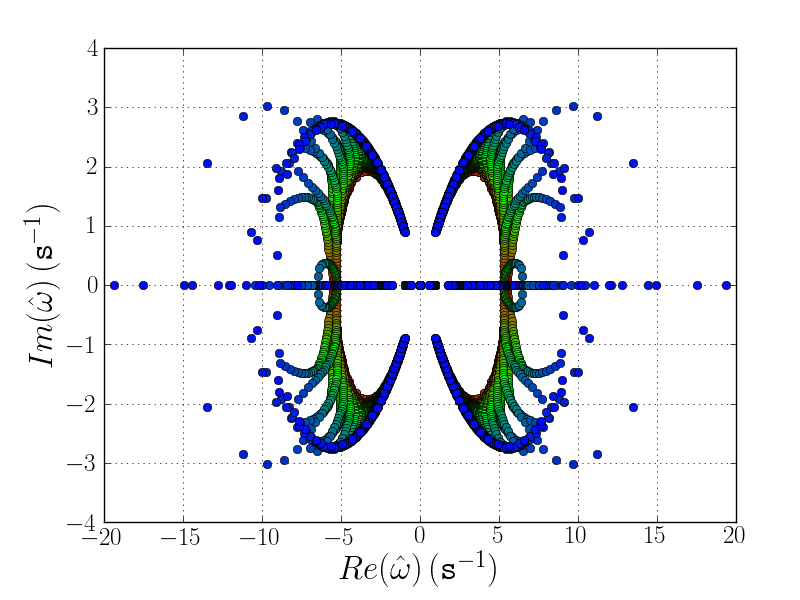
\includegraphics[width=\twofigs]{chapters/lopes/png/L2_dx_0_02_hm_spike_spectrum_StdPot.png}
%%  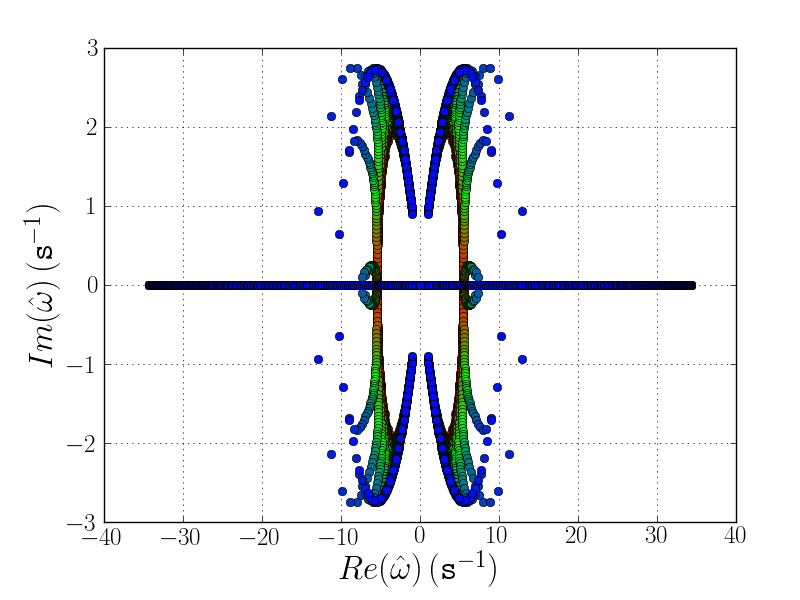
\includegraphics[width=\twofigs]{chapters/lopes/png/L2_dx_0_02_hm_shelf_spectrum_StdPot.png} \\
%%  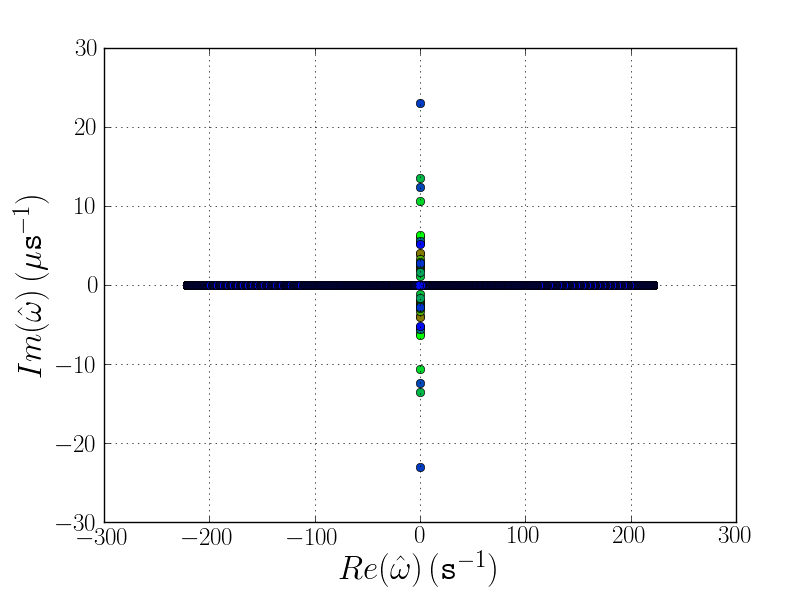
\includegraphics[width=\twofigs]{chapters/lopes/png/L2_dx_0_02_hm_spike_spectrum_Zhao.png}
%%  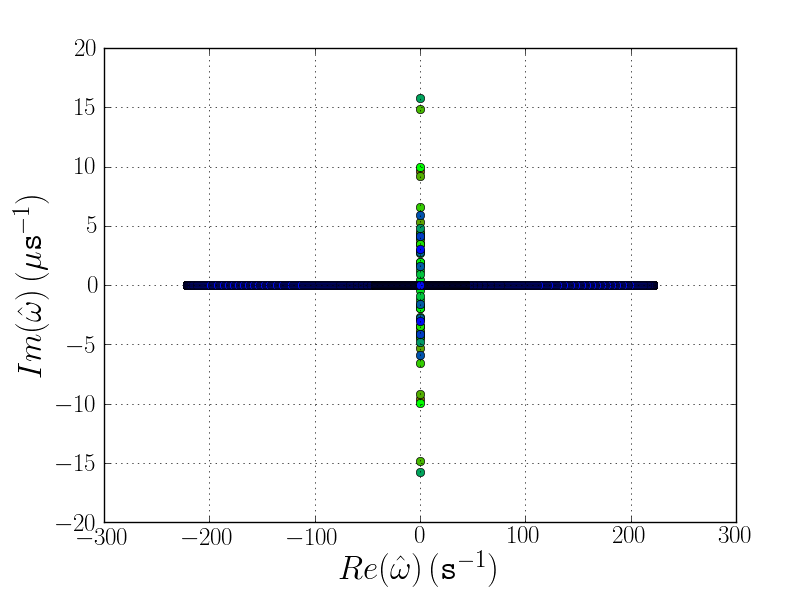
\includegraphics[width=\twofigs]{chapters/lopes/png/L2_dx_0_02_hm_shelf_spectrum_Zhao.png}
\caption{Eigenvalue spectrum for the standard potential (upper
    panels) and ZTC (lower panels) models for the spike (left panels) and
    shelf (right panels) geometries, with $l=2$ {\tt m}, $\Delta
    x~=~0.02$\,~{\tt m} and $h_m$ from $1$~{\tt m} (red circles) to
    $0.02$~{\tt m} (blue circles).}\label{fig:lopes:spectrumhm1}\vspace*{-6pt}
\end{figure}

In Figs. \ref{fig:lopes:spectrumhm1}--\ref{fig:lopes:spectrumhm3}, we
present the eigenvalues for the standard potential (upper panels) and
ZTC (lower panels) models, for the spike (left panels) and shelf
(right panels) geometries, with $l=2$ {\tt m} and $\Delta x=0.02$ {\tt
m}, $l=1$ {\tt m} and $\Delta x=0.1$ {\tt m} as well as $l=0.5$ {\tt
m} and $\Delta x=0.25$ {\tt m}. The spectrum depends on $h_m$ and the
eigenvalues are plotted with different colors (from red to blue) to
accentuate that dependence ($h_m\approx 1$~{\tt m}, $h_m\approx
0.5$~{\tt m} and $h_m\approx 0.02$~{\tt m} denoted by red, green and
blue circles, respectively).



As in~\citet{LovholtPedersen2009}, we find instabilities of type I and
II for the standard potential model, specially for steep bottom
gradients and finer meshes.  We also observe that as $l$ increases so
does the number of unstable wave modes.  Moreover, a steep gradient
increases the growth rate of the unstable solutions for the standard
potential model.  In contrast, for the ZTC model all the growth rates
are limited to $|Im(\hat\omega)|=3\times 10^{-5}\,~{\tt s}^{-1}$.  It
was shown in~\citet{LovholtPedersen2009} that a lower bound growth
rate of $|Im(\hat\omega)|=10^{-5}\,~{\tt s}^{-1}$ does not influence
the numerical results in most real problems, even when steep bottom
gradients occur as in tsunami simulations.

\begin{figure}[!t]
%\bwfig
  \centering
\includegraphics{0001335358/272415_1_en_25_fig9_print.tif}
%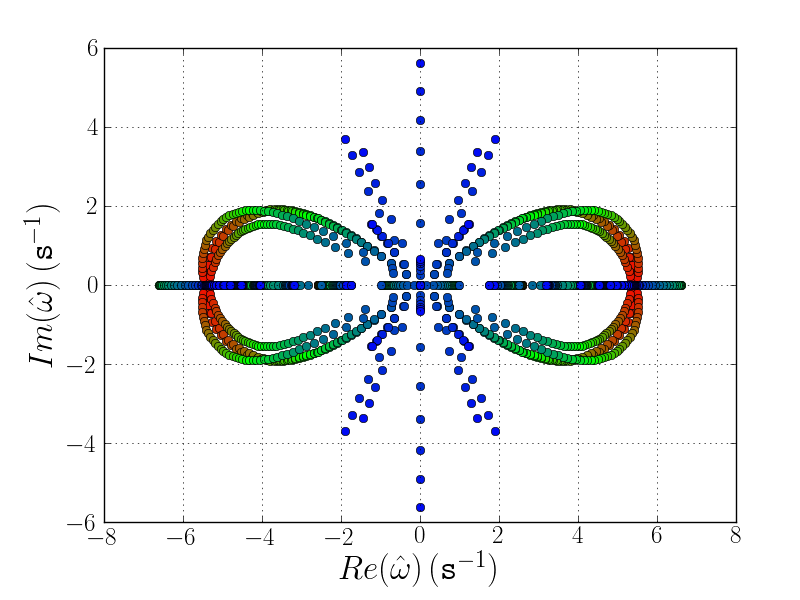
\includegraphics[width=\twofigs]{chapters/lopes/png/L1_dx_0_1_hm_spike_spectrum_StdPot.png}
%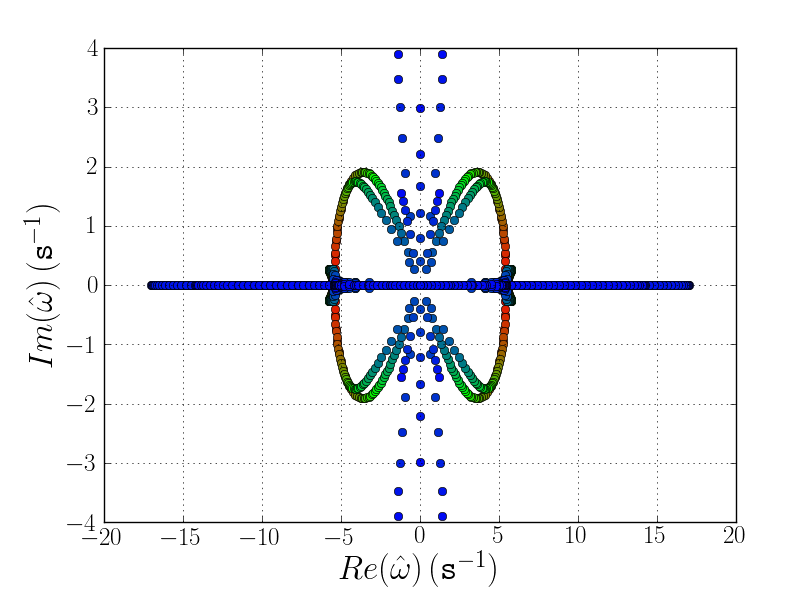
\includegraphics[width=\twofigs]{chapters/lopes/png/L1_dx_0_1_hm_shelf_spectrum_StdPot.png} \\
%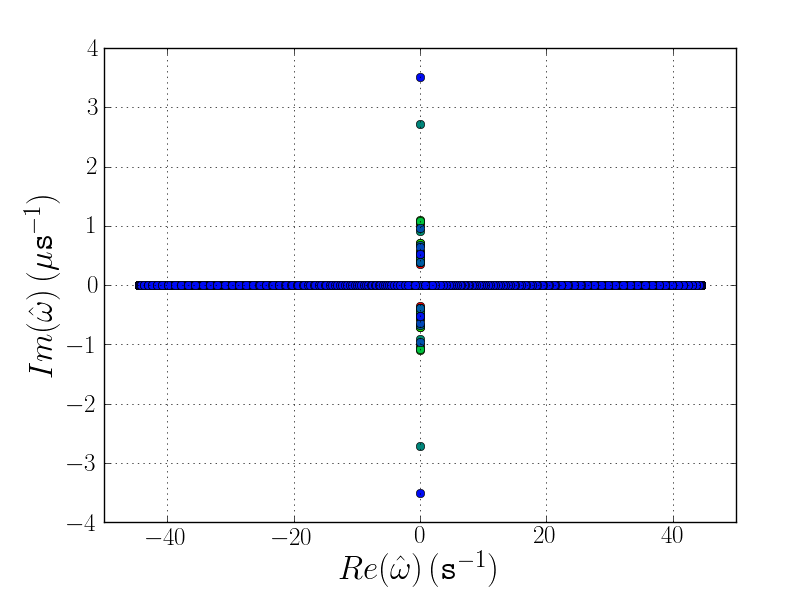
\includegraphics[width=\twofigs]{chapters/lopes/png/L1_dx_0_1_hm_spike_spectrum_Zhao.png}
%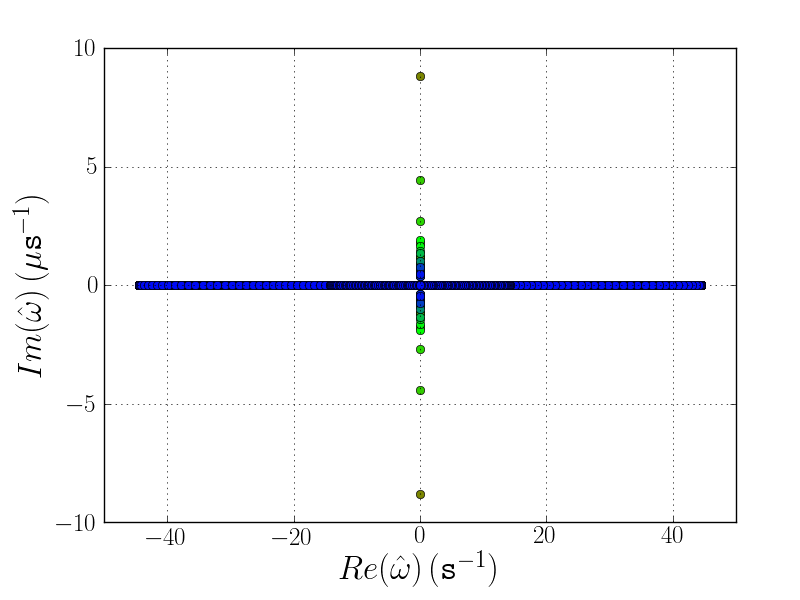
\includegraphics[width=\twofigs]{chapters/lopes/png/L1_dx_0_1_hm_shelf_spectrum_Zhao.png}
  \caption{Eigenvalue spectrum for the standard potential (upper
    panels) and ZTC (lower panels) models for the spike (left panels) and
    shelf (right panels) geometries, with $l=1$ {\tt m}, $\Delta
    x~=~0.1$\,~{\tt m} and $h_m$ from $1$~{\tt m} (red circles) to
    $0.02$~{\tt m} (blue circles).}
  \label{fig:lopes:spectrumhm2}\vspace*{10pt}
\end{figure}

\begin{figure}[!t]
%\bwfig
  \centering
\includegraphics{0001335358/272415_1_en_25_fig10_print.tif}
  %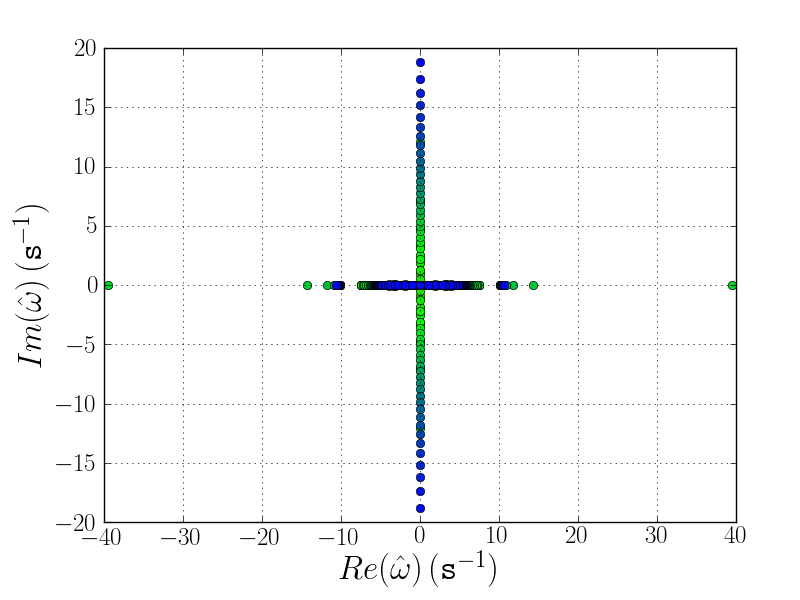
\includegraphics[width=\twofigs]{chapters/lopes/png/L0_5_dx_0_25_hm_spike_spectrum_StdPot.png}
  %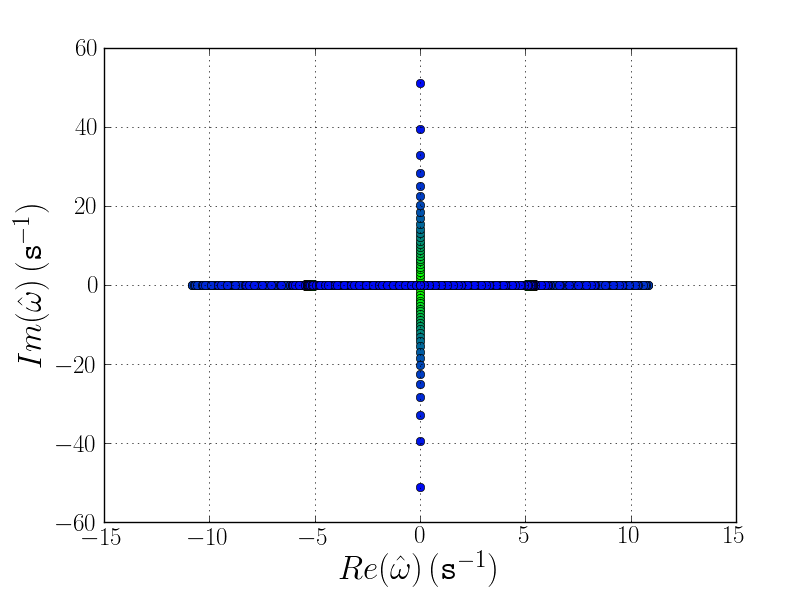
\includegraphics[width=\twofigs]{chapters/lopes/png/L0_5_dx_0_25_hm_shelf_spectrum_StdPot.png} %\\
  %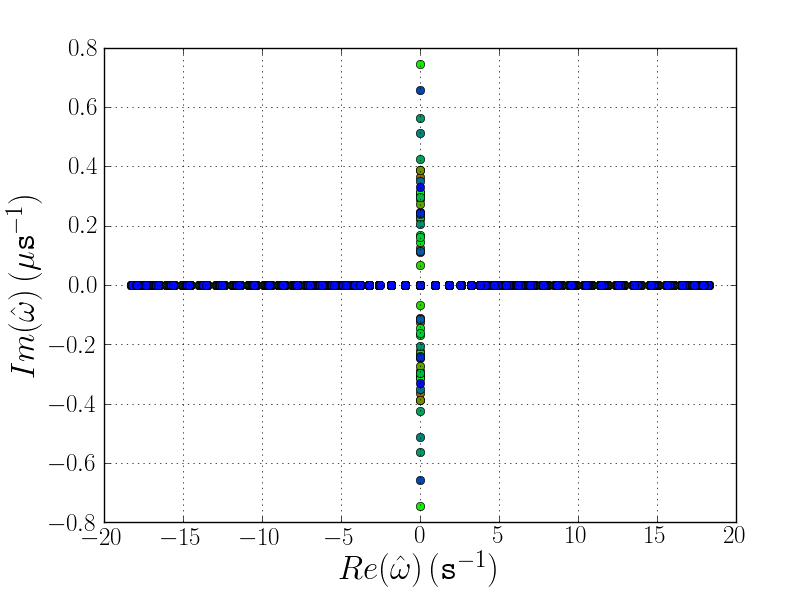
\includegraphics[width=\twofigs]{chapters/lopes/png/L0_5_dx_0_25_hm_spike_spectrum_Zhao.png}
  %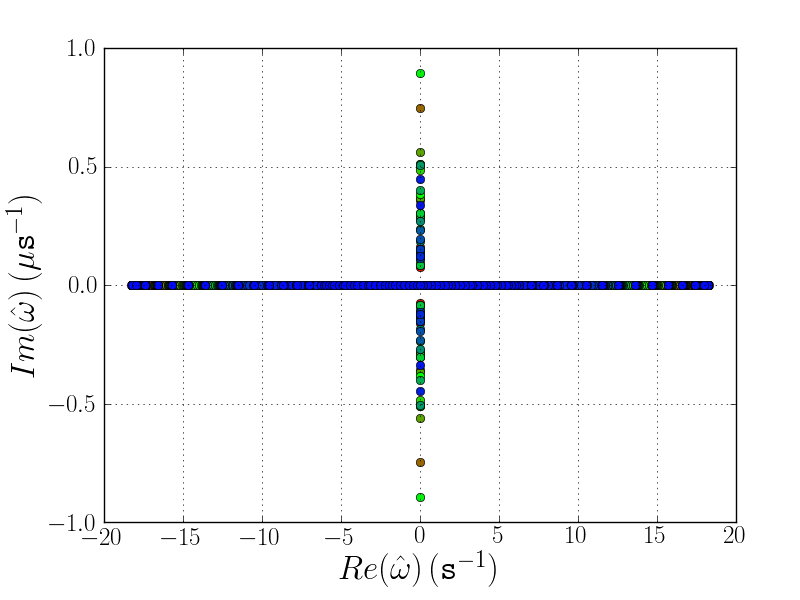
\includegraphics[width=\twofigs]{chapters/lopes/png/L0_5_dx_0_25_hm_shelf_spectrum_Zhao.png}
\caption{Eigenvalue spectrum for the standard potential (upper
    panels) and ZTC (lower panels) models for the spike (left panels) and
    shelf (right panels) geometries, with $l=0.5$ {\tt m}, $\Delta
    x~=~0.25$\,~{\tt m} and $h_m$ from $1$~{\tt m} (red circles) to
    $0.02$~{\tt m} (blue circles).}
  \label{fig:lopes:spectrumhm3}
\end{figure}


From Figures \ref{fig:lopes:spectrum1}--\ref{fig:lopes:spectrumhm3},
we can conclude that the ZTC model is very robust in terms of the
instabilities depending on $l$, depth gradients and mesh
discretizations.

In the next section, we also test the weakly nonlinear ZTC model in
order to verify its robustness with respect to instabilities.

\vspace*{5pt}
\section{Model validation and numerical applications}
\label{sec:lopes:numericaltests}

To validate the model we consider two benchmark tests.  Additionally,
the wave propagation in a harbor as well as the generation of a wave
due to a time dependent moving bottom are also investigated.

\vspace*{3pt}
\subsection{Solitary wave over  submerged bars}

In this subsection, we simulate the propagation of a solitary wave
passing through trapezoidal and triangular submerged bars.  Moreover,
the solutions obtained by the DOLFWAVE (ZTC/BEP) solver are compared
with those provided by a \fenics independent numerical code to solve
the Nwogu's BEV equations (see \emp{dolfwave/tools/Nwogu}).
Specifically, a finite element discretization of these Nwogu's
equations is considered (see~\citet{Walkley1999}) together with an
implicit Radau IIA-type Runge--Kutta scheme for the time integration
(see~\citet{HairerWanner1991b}).

We start now the description of the problem along with the DOLFWAVE
code used to solve it. This C++ code should start with the inclusion
of the DOLFWAVE library.\vspace*{2pt}
%%
\begin{c++}
#include <dolfwave.h>
using namespace dolfin::dolfwave;
\end{c++}

\vspace*{5pt}

\noindent The initial condition for the wave surface elevation is
given by~\eqref{eq:lopes:solita} and implemented as follows:\vspace*{2pt}
\begin{c++}
class ElevationInit : public Expression
{
  void eval(Array<double> & values,const Array<double> & x) const
  {
    // Wave parameters (see Walkley [1999])
    double c=sqrt(1.025), H=0.4;
    double ca=-0.4, cb=ca+1.0/3.0;
    double center=-5.0;
    double a1=(H/3.0)*(sqr(c)-1)/(cb-ca*sqr(c));
    double a2=-(H/2.0)*sqr((sqr(c)-1)/c)*(cb+2.0*ca*sqr(c))/(cb-ca*sqr(c));
    double k=(1.0/(2.0*H))*sqrt((sqr(c)-1)/(cb-ca*sqr(c)));
    values[0]=a1/sqr(cosh(k*(x[0]-center)))+a2/sqr(sqr(cosh(k*(x[0]-center))));
  }
};
\end{c++}

\pagebreak

\noindent Moreover, the initial condition for the velocity potential is defined
by~\eqref{eq:lopes:solitp} and implemented using the following code:
%%
\begin{c++}
class PotentialInit :  public Expression
{
  void eval(Array<double> & values,const Array<double> & x) const
  { //Wave parameters
    double c=sqrt(1.025), H=0.4;
    double ca=-0.4, cb=ca+1.0/3.0;
    double center=-5.0;
    double a3=sqrt(H*g_e)*(sqr(c)-1)/c;
    double k=(1.0/(2.0*H))*sqrt((sqr(c)-1)/(cb-ca*sqr(c)));
    double cnst=4.0*a3/(2.0*k*(1+exp(2.0*k*(-25.)))); //Constant of integration
    values[0]=-4.0*a3/(2.0*k*(1+exp(2.0*k*(x[0]-center))))+cnst;
  }
};
\end{c++}
%%

Te trapezoidal sea bottom $h$ ({\tt m}) is described by the following
continuous and piecewise differentiable function:
%%
\begin{align}
  \label{eq:lopes:piecewisebottom}
  h(x)=\begin{cases}
    0.4& {\rm if}\quad -25 \leqslant x\leqslant 6\\
    -0.05x+0.7& {\rm if}\quad 6< x\leqslant 12\\
    0.1& {\rm if}\quad 12< x\leqslant 14\\
    0.1x-1.3& {\rm if}\quad 14< x\leqslant 17\\
    0.4& {\rm if}\quad 17< x\leqslant 25
  \end{cases}  ({\tt m})
\end{align}
%%
which is implemented by:
%%
\begin{c++}
class Depth :  public Expression
{
  void eval(Array<double> & values,const Array<double> & x) const
  {
    double retrn = 0.0;
    if (x[0] <= 6.0)
      retrn=0.4;
    else if (x[0] <= 12.0)
      retrn=-0.05*x[0]+0.7;
    else if (x[0] <= 14.0)
      retrn=0.1;
    else if(x[0] <= 17.0)
      retrn = 0.1*x[0]-1.3;
    else
      retrn = 0.4;
    values[0] = retrn;
  }
};
\end{c++}

The main code starts with the creation of an object of the Dolfwave
class by calling its constructor.  Here, we simulate the wave
propagation during $25$ s using a time step of $0.001$ s.  The \ufl\
form file used in this problem, which is identified by ``Zhao\_1D'',
corresponds to the one horizontal dimensional version
of~\eqref{eq:lopes:varform}.  We use a LU solver provided by the PETSc
algebra backend (see Chapter~\ref{chap:langtangen}).  Here we use
Viper for previewing the numerical solutions, which are saved in the
``output'' directory using a simple ASCII format denoted by ``xyz''.
%%
\begin{c++}
int main( )
{
  Dolfwave dw(25000 /*Number of steps*/,
              0.001 /*Time step*/,
              100 /*Gap for saving the solutions*/,
              "Zhao_1D" /*Variational form identifier*/,
              "LU_P" /*Linear solver type*/,
              "viper" /*Preview program*/,
              "output" /*Output directory*/,
              "xyz" /*File output format*/);
\end{c++}

\vspace*{5pt}

\noindent The spatial domain used in the case of the trapezoidal
submerged bar  is the interval $[-25,25]$ ({\tt m})
which is discretized using 201 nodes.\vspace*{2pt}
%%
\begin{c++}
Interval mesh(201,-25,25);
\end{c++}

\vspace*{5pt}

\noindent Now all the known functions are initialized.  Sponge layers or source
functions are not used here.\vspace*{2pt}
%%
\begin{c++}
Depth depth; // Depth function
ElevationInit eta_init; // Initial condition for the surface elevation
PotentialInit phi_init;  // Initial condition for the velocity potential
Constant zero(0.0); // Sponge layers and source function are 0
\end{c++}

\vspace*{5pt}

\noindent From the bilinear and linear forms of the variational formulation, all
the finite element matrices and vectors are created.\vspace*{2pt}
%%
\begin{c++}
dw.SpacesFunctionsVectorsInit(mesh); // Initialization of the spaces, functions and vectors
dw.BilinearFormInit(mesh,depth); // Initialization of the bilinear form "a"
dw.MatricesAssemble( ); // Initialization of the system matrices
dw.LinearFormsInit(depth, zero, zero, zero, zero, zero); // Initialization of the linear form "L"
dw.InitialCondition(eta_init,phi_init); // Setting the initial conditions
\end{c++}

\vspace*{5pt}

\noindent We only need to make an initial factorization for the LU solver, since
the system matrix does not depend on time.\vspace*{2pt}
%%
\begin{c++}
dw.LUFactorization(true); // Reuse the LU factorization throughout the time integration routines
\end{c++}

\vspace*{5pt}

\noindent The output of the symmetric of the depth function is given by:
%%
\begin{c++}
dw.DepthPlot(mesh,depth,true); // Plot the symmetric of the depth function h
\end{c++}

\vspace*{5pt}

\noindent Now, the time integration routines are used.
The Adams--Bashforth--Moulton method described by
equations~\eqref{eq:lopes:pc} is initialized by a fourth-order explicit
Runge--Kutta scheme.

\pagebreak%

\begin{c++}
dw.RKInit("exp4");    // Choose the explicit 4th-order Runge-Kutta for initialization
dw.RKSolve( );        // Use the Runge-Kutta for the 3 initial steps
dw.PCInit(mesh,true); // Initialization of the predictor-corrector with multi-step corrector

// Advance in time with the predictor-corrector scheme
for(dolfin::uint i=4; i<dw.MaxSteps+1;i++)
{
  dw.PCSolve( ); // Adams-Bashforth-Moulton method
  if (!(i%dw.WriteGap)) // Save and preview the surf. elevation with a gap of 100 iterations

  dw.Plot(mesh, true /*eta preview*/, false /*phi preview*/,
          true /*eta save*/, false /*phi save*/);
}
\end{c++}%\vspace*{10pt}
%%
In this case only the wave surface elevation is saved and previewed
using the Plot function.  The solution provided by this code, for the
trapezoidal submerged bar with $x\in[-10,25]$ ({\tt m}), is given in
Figure~\ref{fig:lopes:submergedbar}.  We remark that the shoaling
effect over the trapezoidal submerged bar is clearly observed, both
for the incident and reflected waves.

\begin{figure}[!t]
\centering
\includegraphics{0001335358/272415_1_en_25_fig11_print.eps}
\caption{Detailed view of a wave passing through a trapezoidal
submerged bar using the ZTC/BEP model implemented in DOLFWAVE}
\label{fig:lopes:submergedbar}
\end{figure}

From Figure~\ref{fig:lopes:zhaonwogu}, we can compare the solutions
provided by the two independent models.  We remark that
~\eqref{eq:lopes:solita} and~\eqref{eq:lopes:solitb} are used for the
correspondent initial conditions of Nwogu's equations.  In spite of
the fact that the solutions come from different models and
discretizations, a good agreement is achieved.  These solutions also
compare well with those provided by another model in the DOLFWAVE
application (see also \emp{dolfwave/demo/1HD/submergedbar}).

\begin{figure}[!t]
%\bwfig
  \centering
  %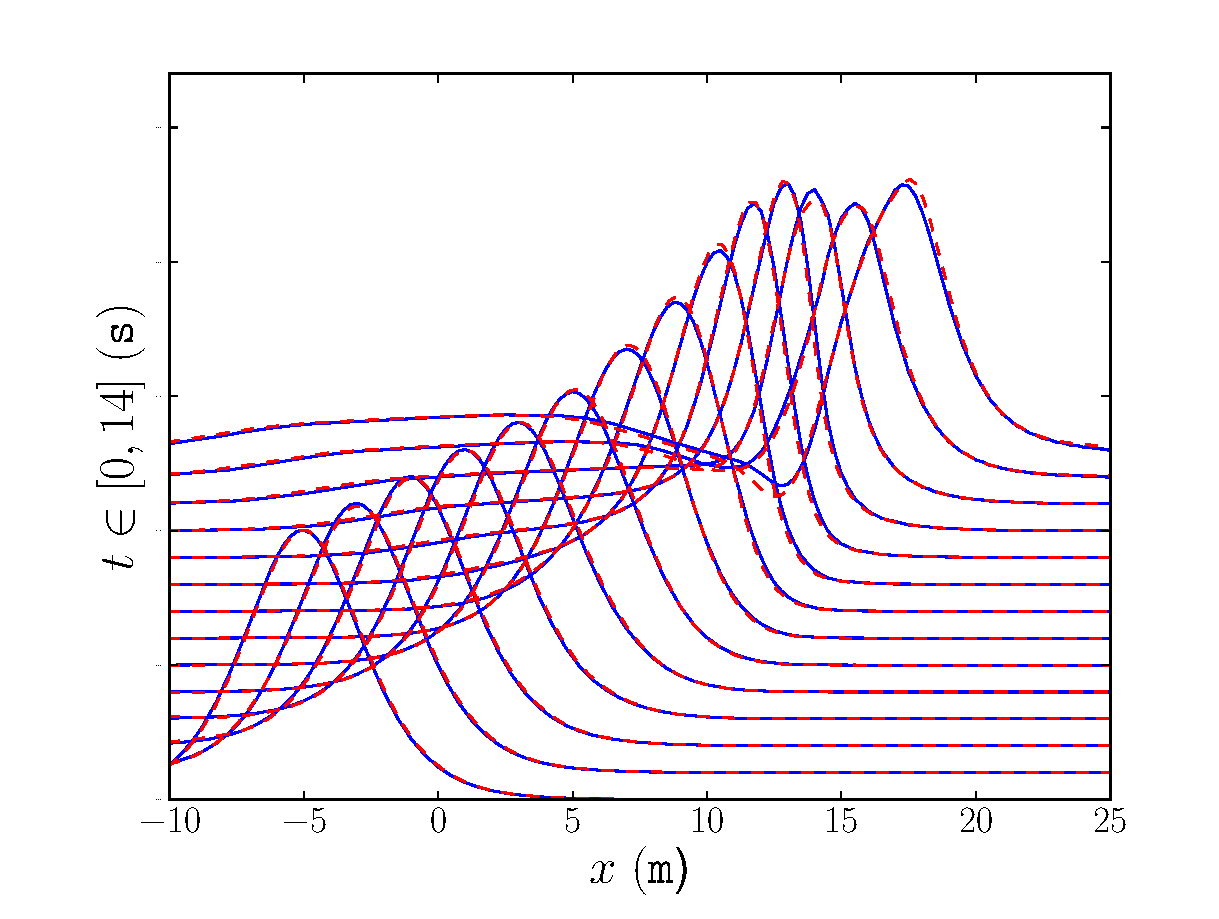
\includegraphics[width=\largefig]{chapters/lopes/pdf/ZhaoNwogu.pdf}
  \includegraphics{0001335358/272415_1_en_25_fig12_print.eps}
  \caption{Detailed comparison of a wave passing through the
    trapezoidal submerged bar, simulated by DOLFWAVE using the ZTC/BEP
    (red dashed line) and Nwogu's BEV (blue solid line) models, for
    $x\in[-10,25]$~({\tt m}) and $t\in[0,14]$~({\tt s}).}
  \label{fig:lopes:zhaonwogu}\vspace*{6pt}
%\vspace*{40pt}
\end{figure}

\begin{figure}[!t]
%\bwfig
  \centering
  %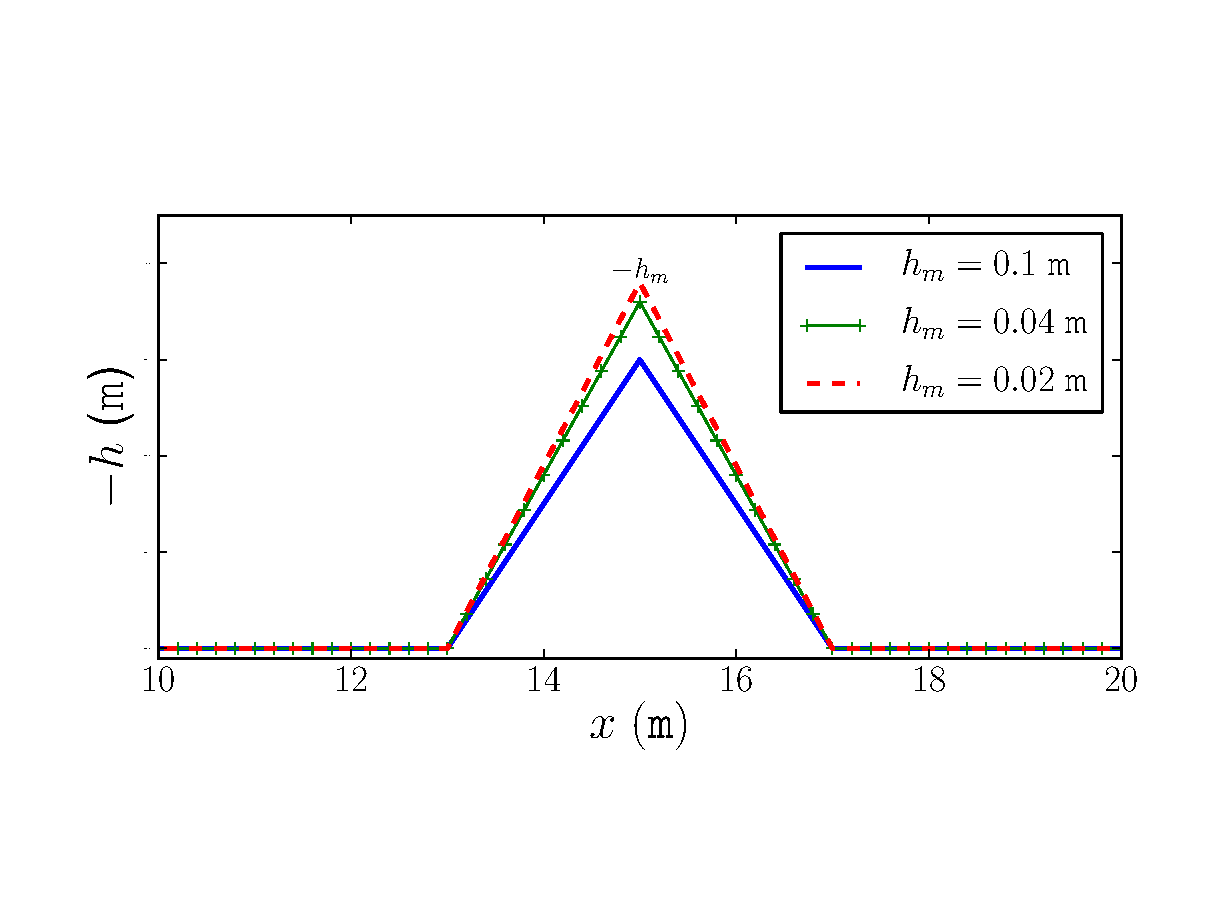
\includegraphics[width=\largefig]{chapters/lopes/pdf/deptheps.pdf}
  \includegraphics{0001335358/272415_1_en_25_fig13_print.eps}
  \caption{Sketch of the three sea bottoms with triangular
    configurations of height $h_m=0.1$~{\tt m} and $\varepsilon=0.1$ (blue
    solid line), $h_m=0.04$~{\tt m} and $\varepsilon=0.25$ (green line
    with plus markers) as well as $h_m=0.02$~{\tt m} and $\varepsilon=0.5$
    (red dashed line).}\label{fig:lopes:spikes}\vspace*{6pt}
\end{figure}

\begin{figure}[t!]
\centering
\includegraphics{0001335358/272415_1_en_25_fig14_print.eps}
  \caption{The detailed comparison of a wave passing through the
  triangular submerged bar with $h_m=0.1$~{\tt m}, $\varepsilon=0.1$,
  $x\in[-25,50]$~({\tt m}) and $t\in[0,25]$~({\tt s}).  These solutions
  are provided by DOLFWAVE using the ZTC/BEP (red dashed line) and
  Nwogu's BEV (blue solid line) models.}
  \label{fig:lopes:znspike01}\vspace*{-6pt}
\end{figure}


In the numerical simulation of a solitary wave passing through the
triangular submerged bar, we~investigate the nonlinear effects and the
influence of $h_m$ (see Figure~\ref{fig:lopes:spikes}) for the weakly
nonlinear ZTC/BEP and Nwogu's BEV models.  From
Figure~\ref{fig:lopes:znspike01} we can conclude that these two models
compare well in the case of the triangular submerged bar with
$h_m=0.1$~{\tt m}.  Even though both models compare well for the
triangular submerged bar with a smaller value of $h_m=0.04$~{\tt m},
the Nwogu's BEV model presents small amplitude and high frequency
oscillations after the interaction with the bar (see
Figure~\ref{fig:lopes:znspike025}).  As the value of $h_m$ is
decreased the Nwogu's model becomes unstable (see
Figure~\ref{fig:lopes:zn05}).  In Figure~\ref{fig:lopes:zn05} the
blowup of the solution provided by the Nwogu's model is observed for
$h_m=0.02$~{\tt m}.  We remark that the reference values of
$\varepsilon$ at the point $(15,-h_m)$ ({\tt m}) are
$\varepsilon=0.1$, $\varepsilon=0.25$ and $\varepsilon=0.5$ for
$h_m=0.1$~{\tt m}, $h_m=0.04$\,~{\tt m} and $h_m=0.02$\,~{\tt m},
respectively. Although, $\varepsilon=0.5$ is clearly out of the range
of validity of both ZTC/BEP and Nwogu's BEV models, the first one
seems more robust when dealing with the nonlinear effects. These
stability properties of the ZTC/BEP model are also observed in
numerical tests involving grid refinements.

\begin{figure}[t!]
%\bwfig
  \centering
  %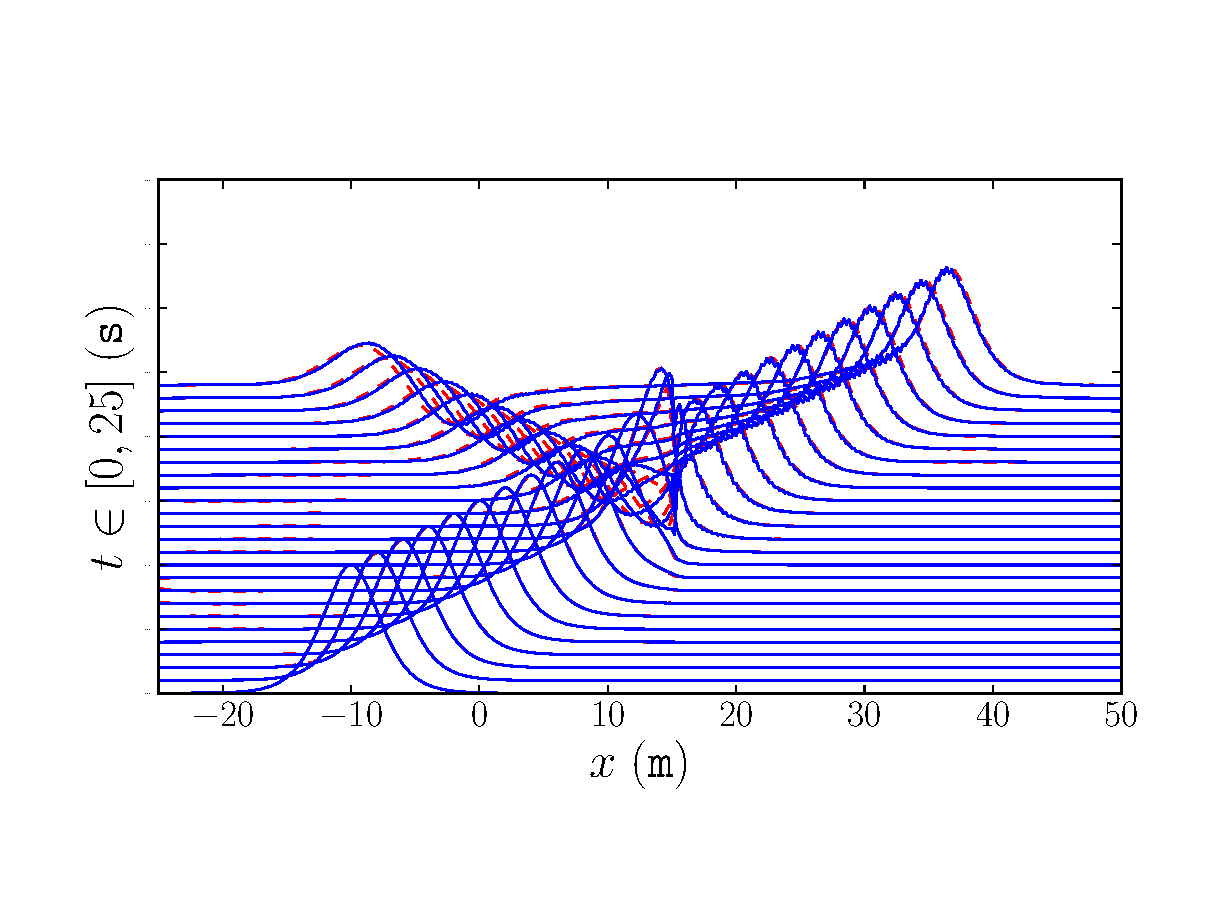
\includegraphics[width=\largefig]{chapters/lopes/pdf/epsilon0_25.pdf}
  \includegraphics{0001335358/272415_1_en_25_fig15_print.eps}
  \caption{The detailed comparison of a wave passing through the
    triangular submerged bar with $h_m=0.04$~{\tt m}, $\varepsilon=0.25$,
    $x\in[-25,50]$~({\tt m}) and $t\in[0,25]$~({\tt s}).  These solutions
    are provided by DOLFWAVE using the ZTC/BEP (red dashed line) and
    Nwogu's BEV (blue solid line) models.  Small amplitude and high
    frequency oscillations are observed in the Nwogu's BEV model
    solutions.}
  \label{fig:lopes:znspike025}\vspace*{9pt}
\end{figure}%\clearpage


\begin{figure}[!t]
%\bwfig
  \centering
  %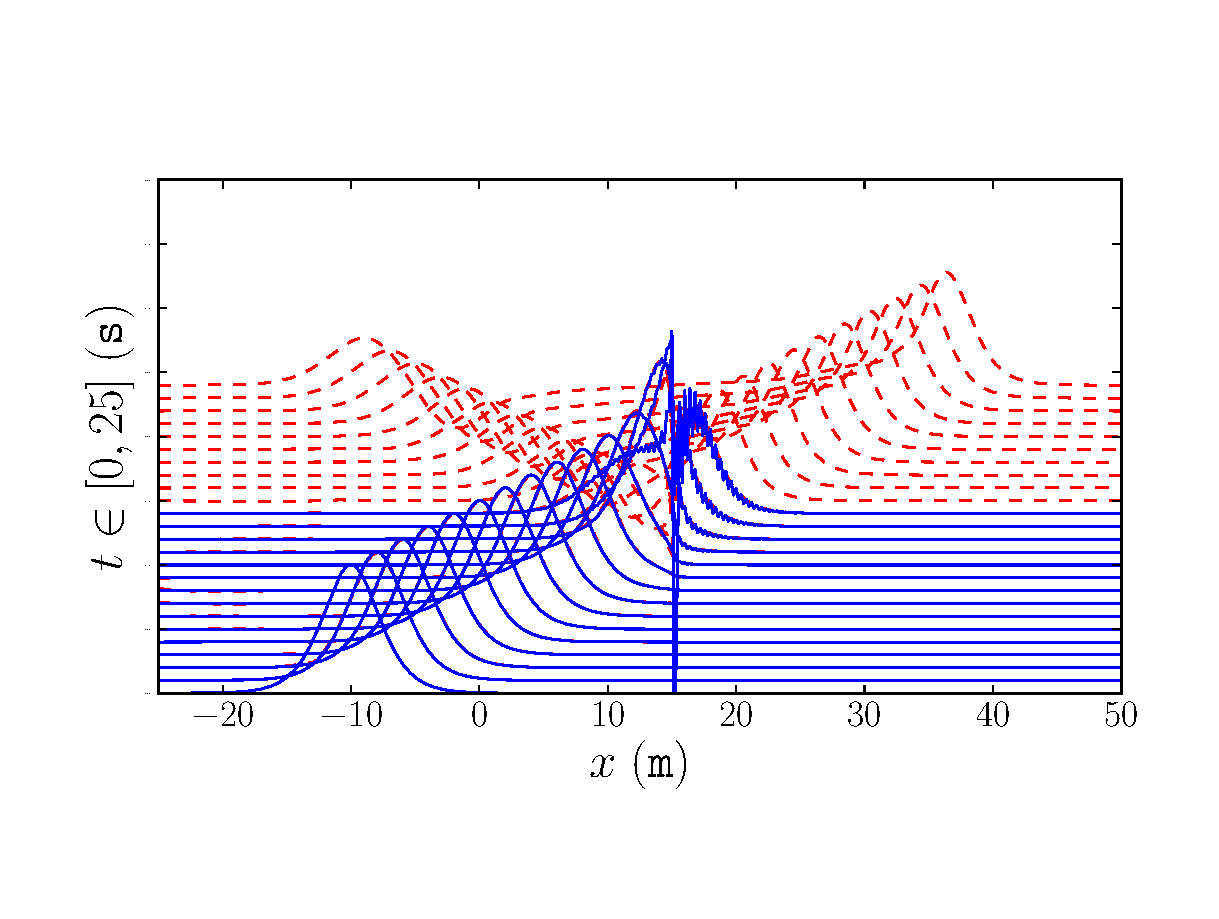
\includegraphics[width=\largefig]{chapters/lopes/pdf/epsilon0_5.pdf}
  \includegraphics{0001335358/272415_1_en_25_fig16_print.eps}
  \caption{The detailed comparison of a wave passing through the
    triangular submerged bar with $h_m=0.02$~{\tt m}, $\varepsilon=0.5$,
    $x\in[-25,50]$~({\tt m}) and $t\in[0,25]$~({\tt s}).  These solutions
    are provided by DOLFWAVE using the ZTC/BEP (red dashed line) and
    Nwogu's BEV (blue solid line) models.  The blowup of the solution
    provided by the Nwogu's BEV model is observed.}
  \label{fig:lopes:zn05}\vspace*{1.5pt}
\end{figure}

\subsection{A Gaussian hump in a square basin}
Here, we simulate the evolution of a Gaussian hump in a square
basin. Analogous tests are available in the literature (see,
e.g.,~\citet{WeiKirby1995} and ~\citet{WooLiu2004a}).  The
computational domain is a square of \(10\times 10\) {\tt m}\(^2\)
which is discretized using triangular unstructured meshes.  Moreover,
we provide grid refinement tests to ensure convergence and accuracy.
Reflective wall boundary conditions are applied
(see~\eqref{eq:lopes:fullrefl}) and no sponge layers are considered.
As initial conditions, we have\vspace*{4pt}
%%
\begin{align}
  \left\{
    \begin{array}{l}
      \eta(x,y,0)=0.1\,e^{-0.4\left((x-5)^2+(y-5)^2\right)}\, \quad
      {(\tt m)},\\[4pt]
      \Phi(x,y,0)=0\,\quad ({\tt m}^2\,{\tt s}^{-1}).
    \end{array}
  \right.%\vspace*{4pt}
\end{align}
%%
A constant depth \(h=0.5\)~{\tt m} is considered.  These initial
conditions and see bottom are considered in the FUNWAVE manual
(see~\citet{Kirby1998}).  Even though we do not know the exact
solutions of the nonlinear equations, the symmetric characteristics of
the problem should result in symmetric surface elevation profiles.
These symmetric properties are conserved in the numerical solutions
provided by DOLFWAVE even for nonsymmetric unstructured meshes.  As an
example, we show in Figure~\ref{fig:lopes:symmetry} the isovalues of
the wave surface elevation for a mesh with $1873$ nodes and
$t=0$\,~{\tt s}, $t=10$\,~{\tt s}, $t=20$\,~{\tt s}, $t=30$\,~{\tt s},
$t\approx 40$\,~{\tt s} as well as $t\approx 50$\,~{\tt s}.  Moreover,
the volume conservation condition is satisfied with a neglectable
error.

\begin{figure}[!t]
  \centering
    %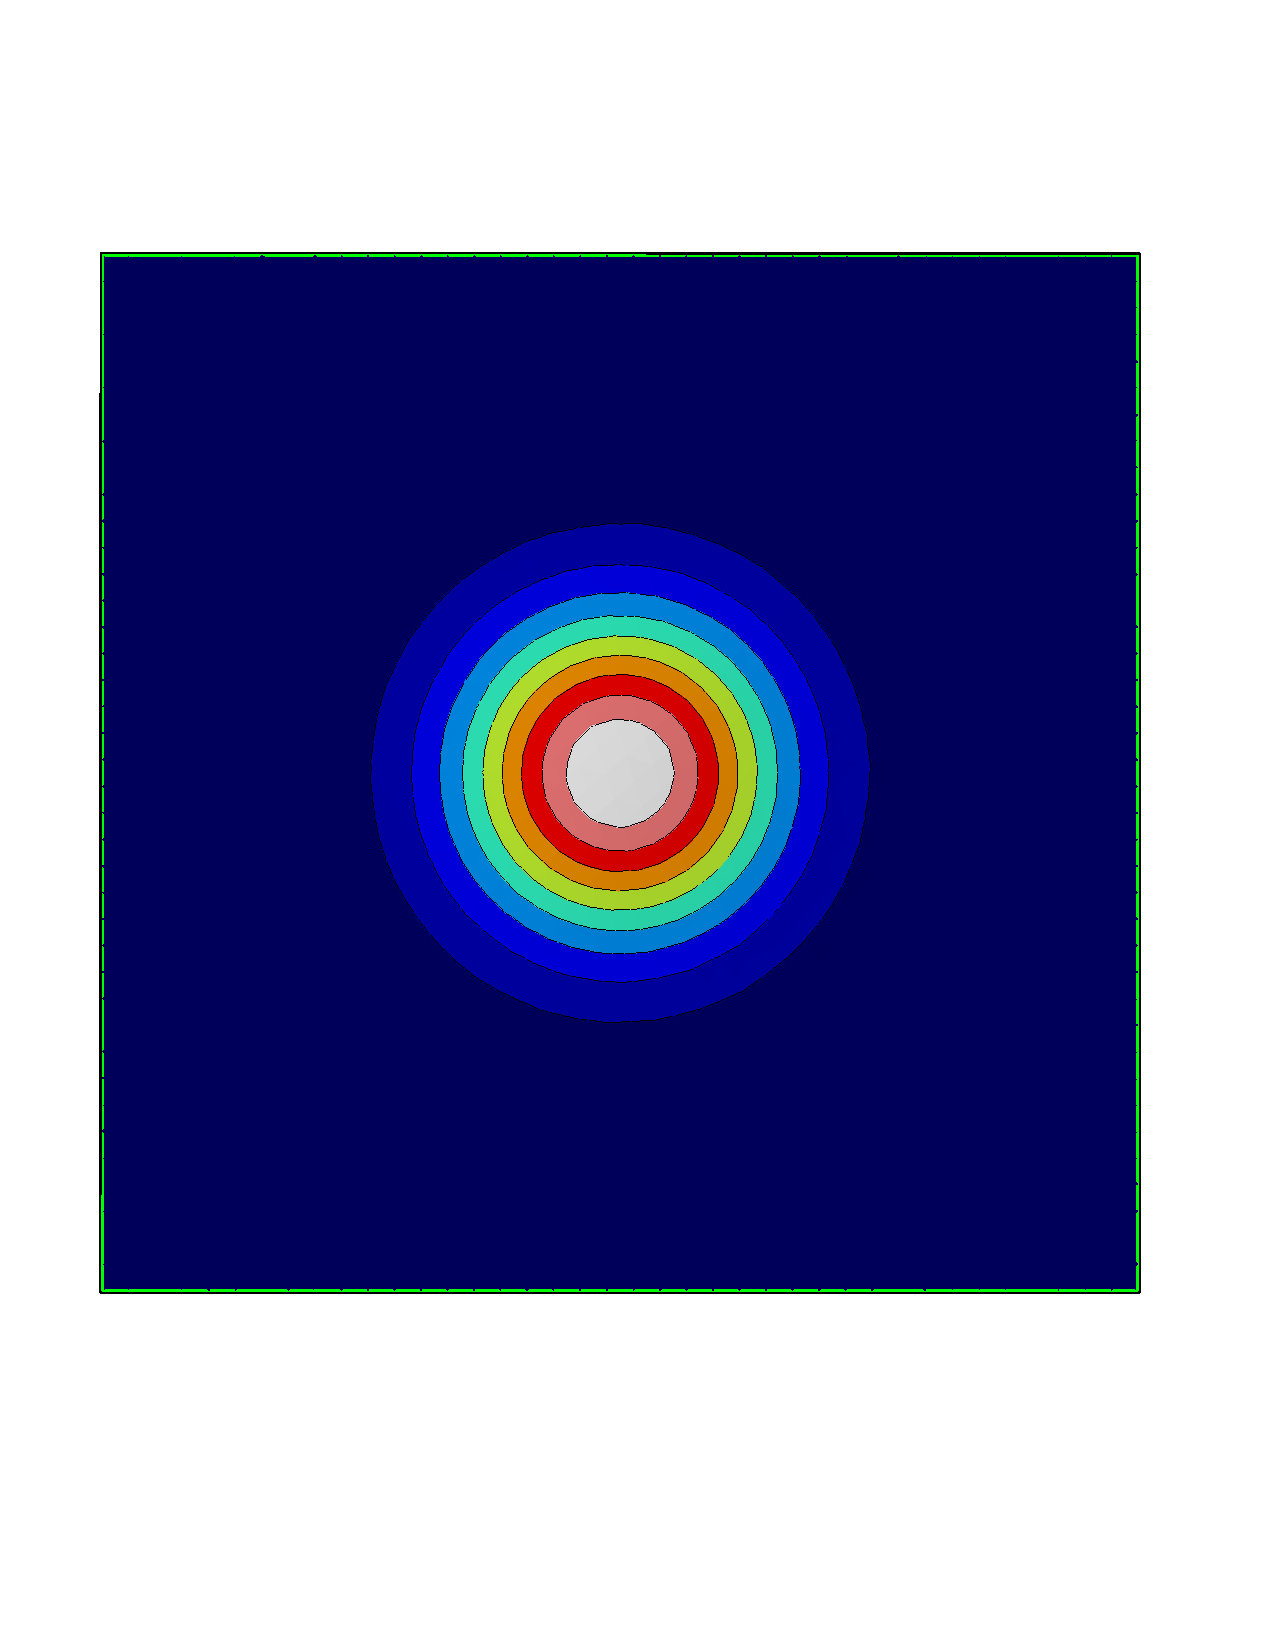
\includegraphics[width=\twofigs]{chapters/lopes/pdf/eta000000.pdf}
    %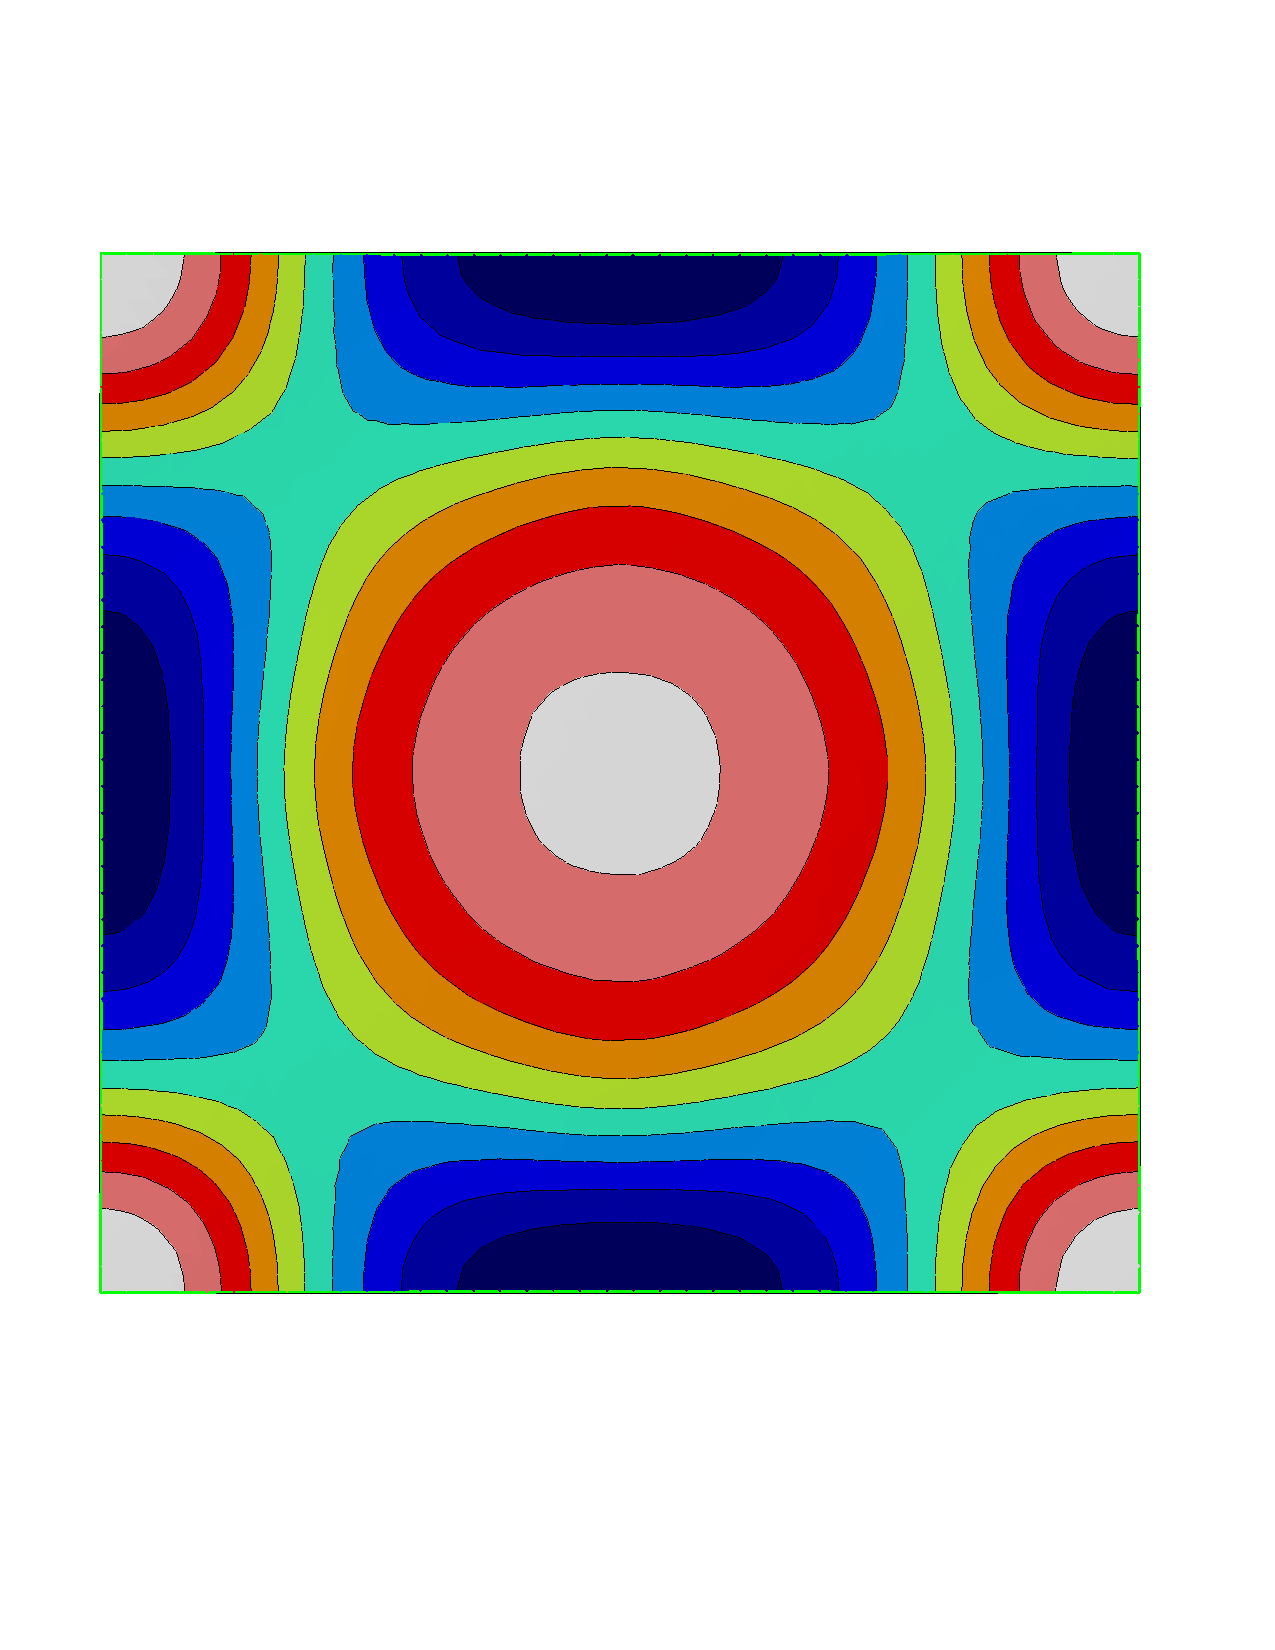
\includegraphics[width=\twofigs]{chapters/lopes/pdf/eta002000.pdf} \\
    %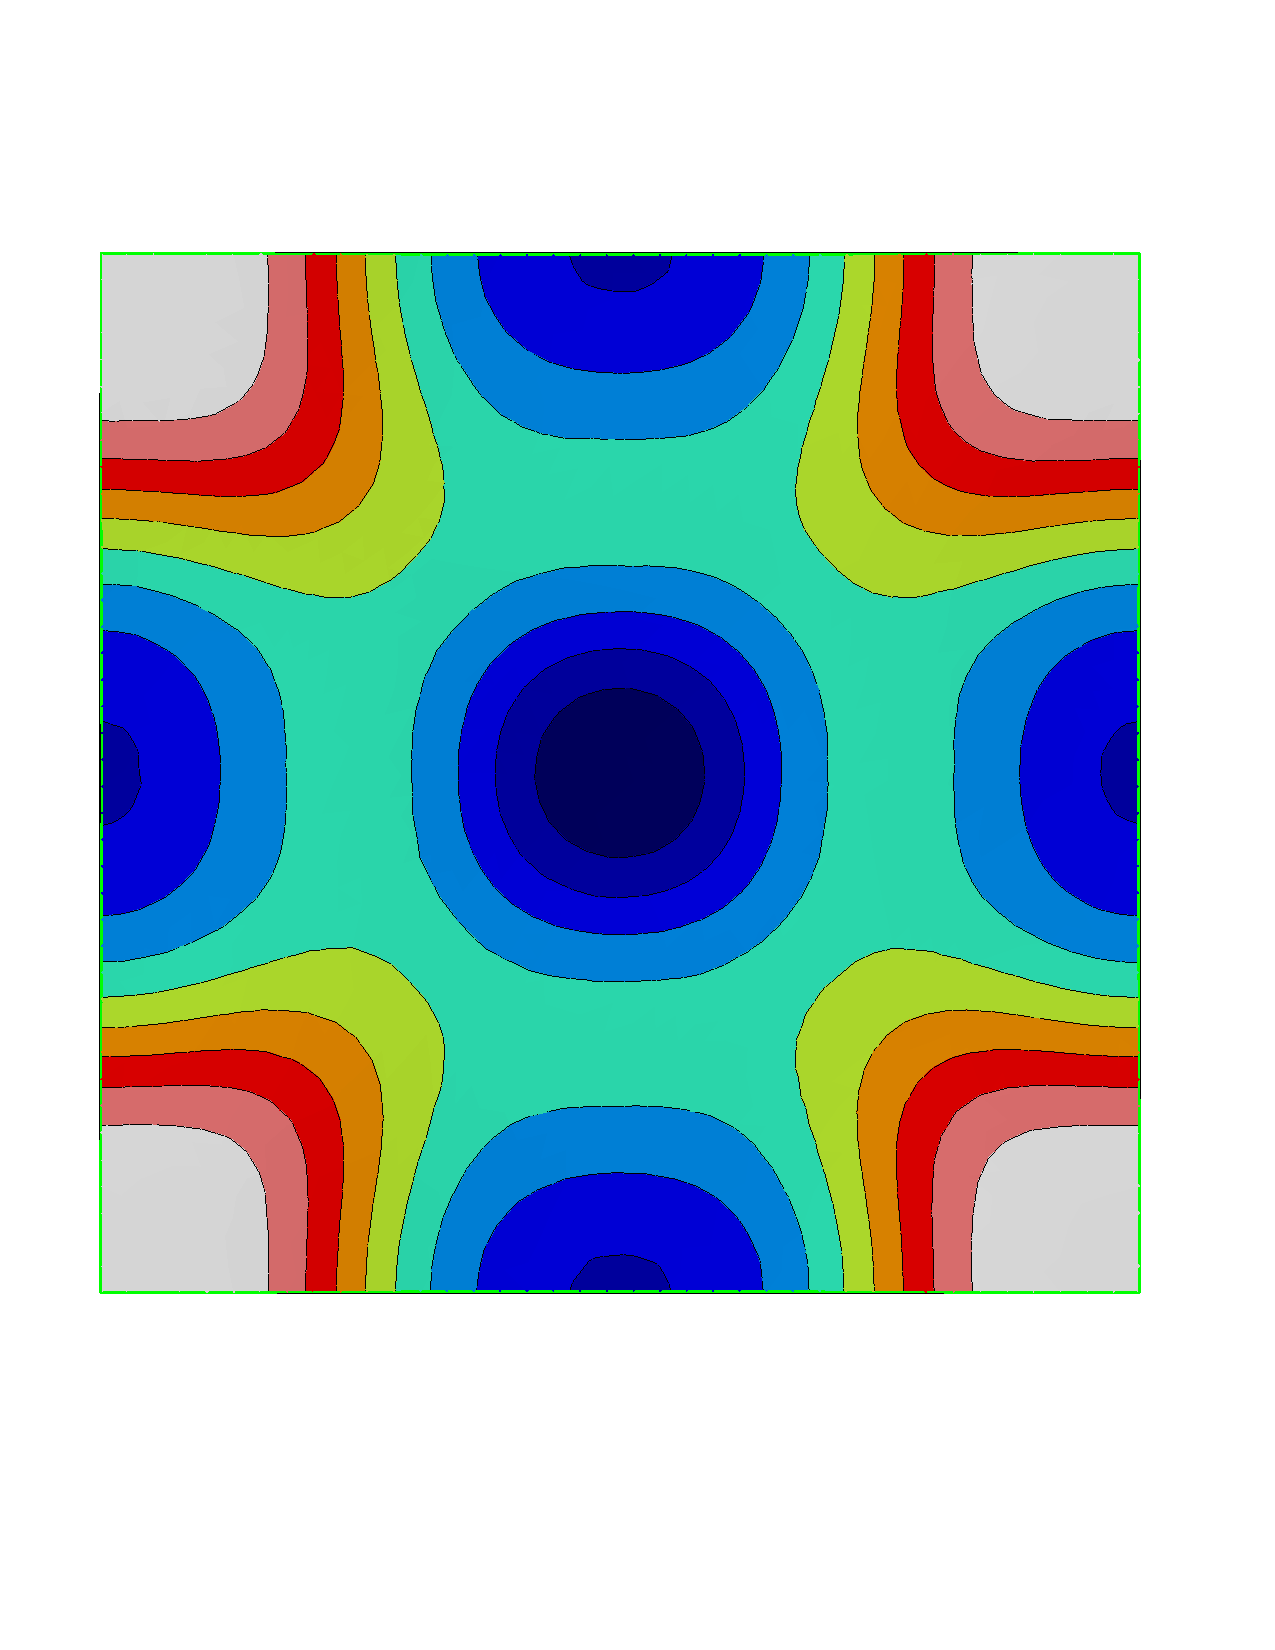
\includegraphics[width=\twofigs]{chapters/lopes/pdf/eta004000.pdf}
    %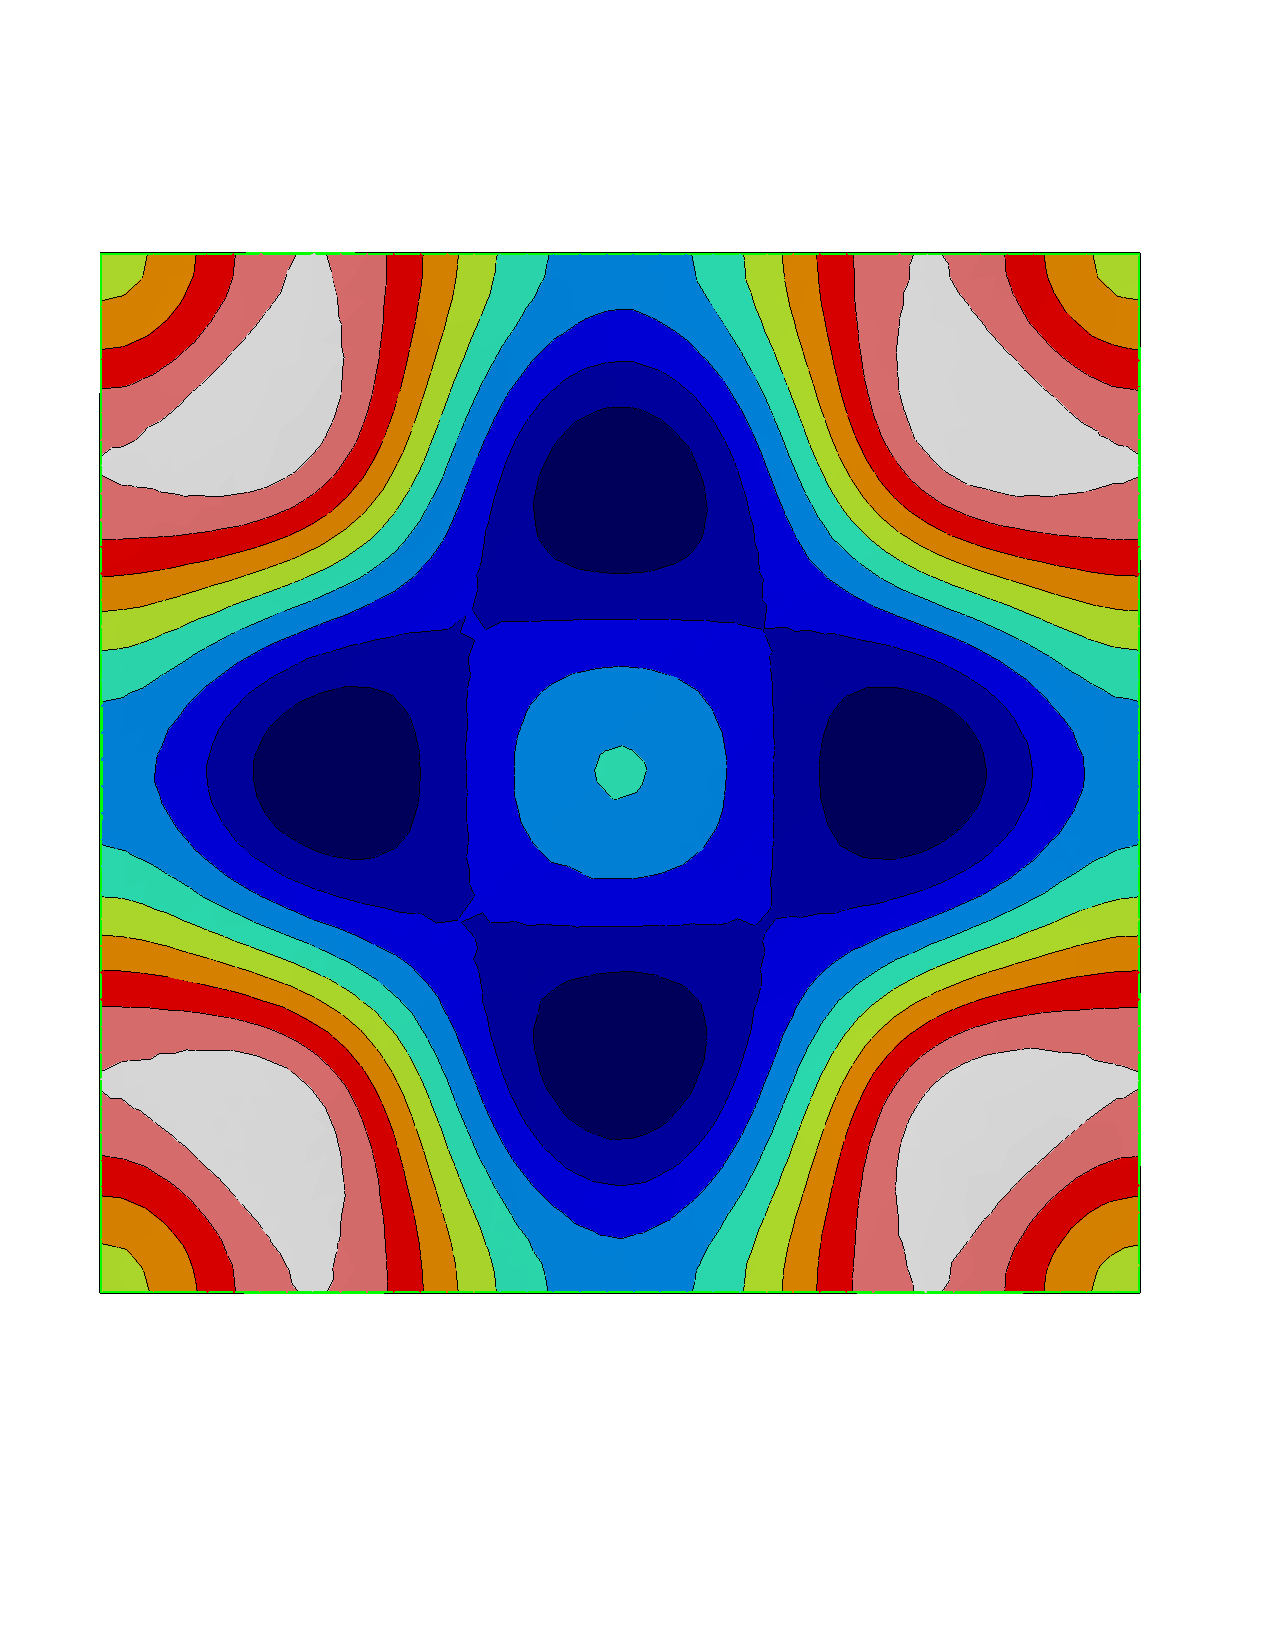
\includegraphics[width=\twofigs]{chapters/lopes/pdf/eta006000.pdf} \\
    %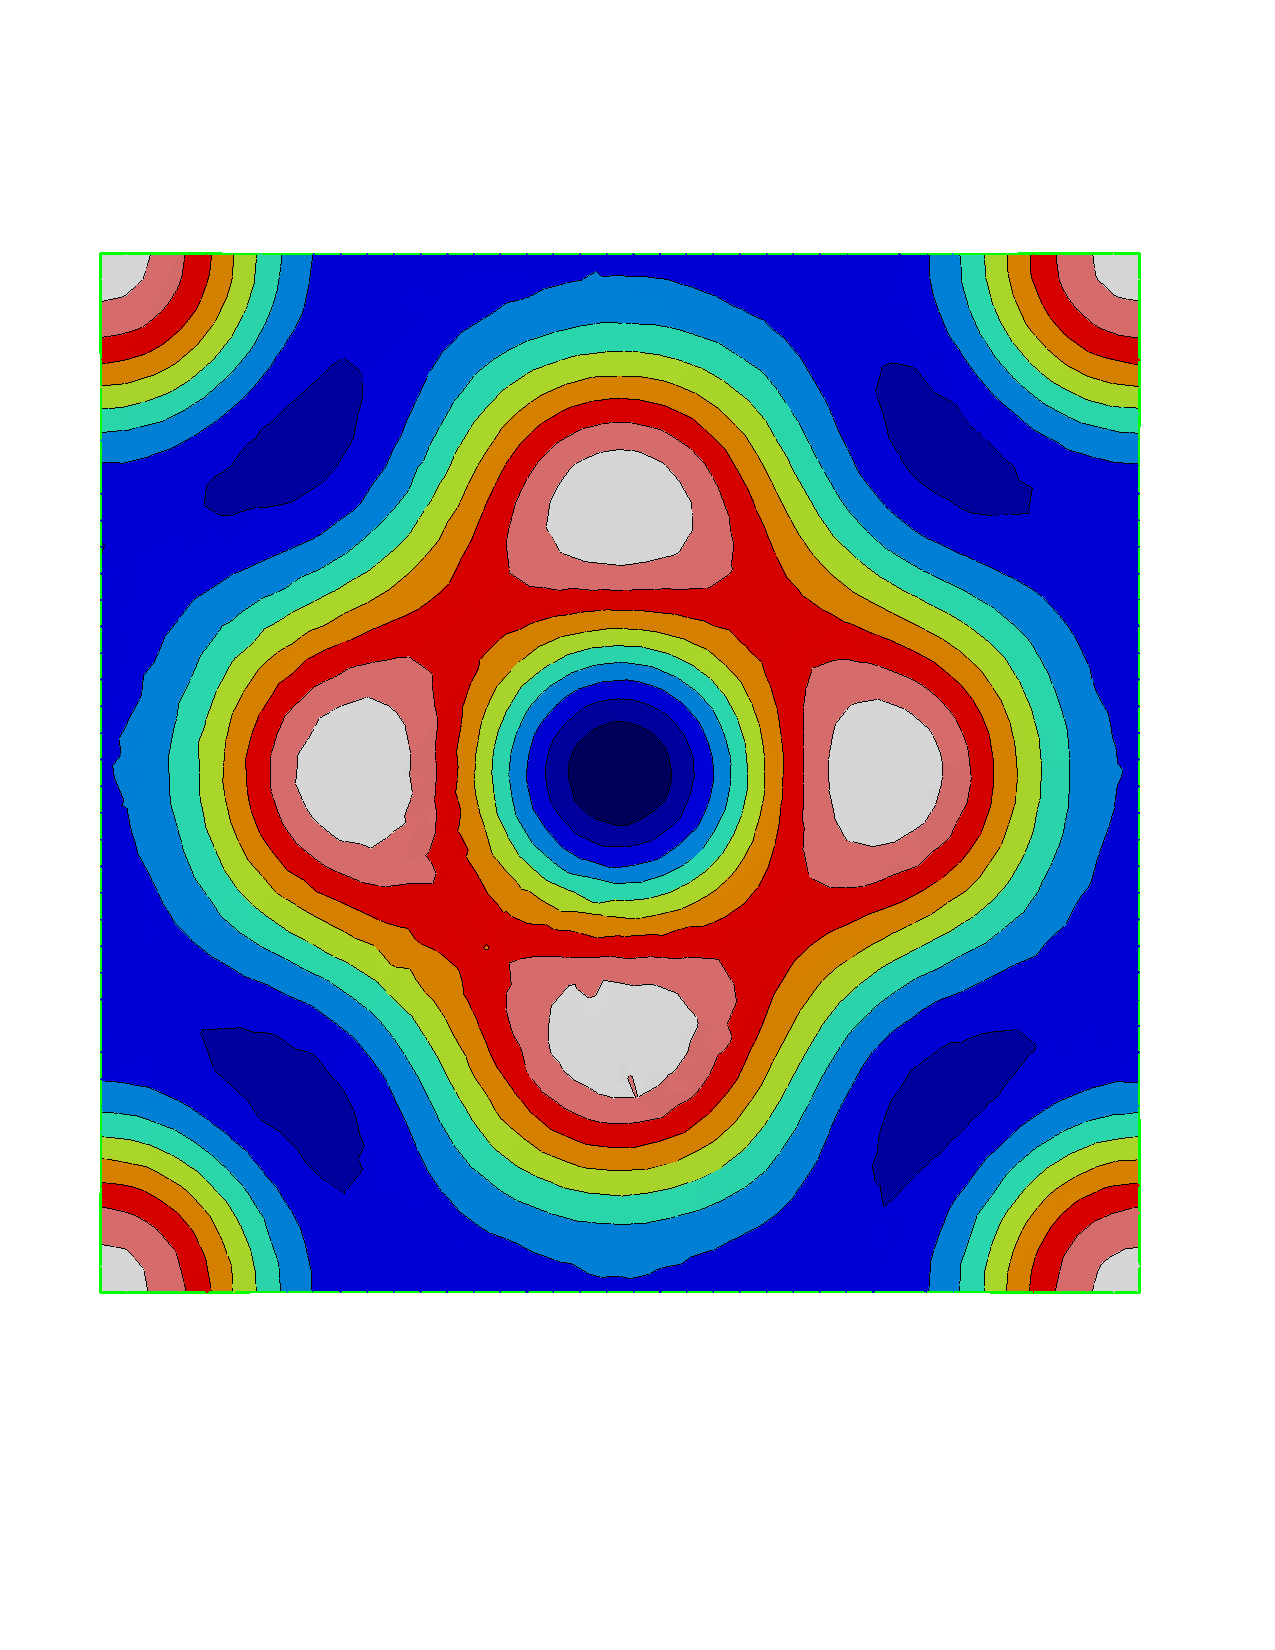
\includegraphics[width=\twofigs]{chapters/lopes/pdf/eta007972.pdf}
    %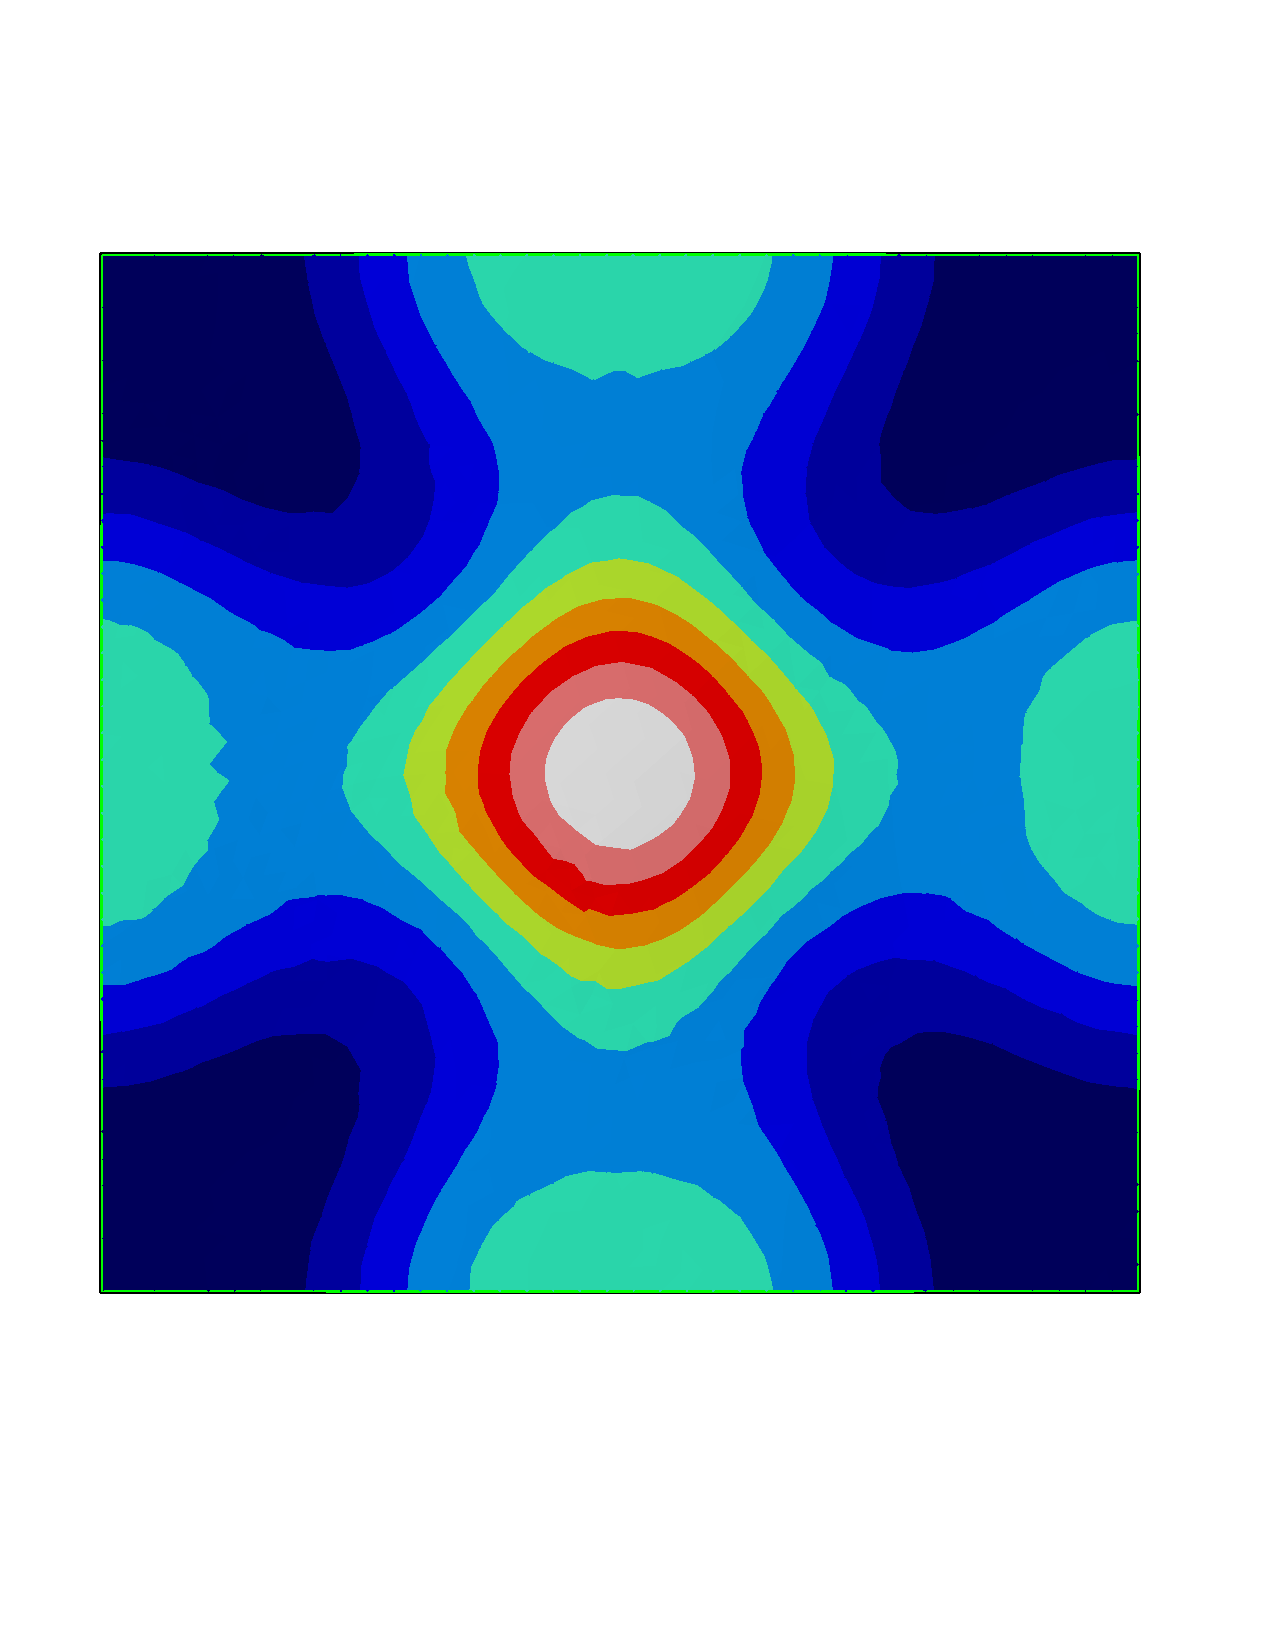
\includegraphics[width=\twofigs]{chapters/lopes/pdf/eta009946.pdf}
    \includegraphics{0001335358/272415_1_en_25_fig17_print.tif}
    \caption{The isovalues of the wave surface elevation $\eta$\,~{\tt
        (m)} at the time $t=0$~{\tt s}, $t=10$~{\tt s}, $t=20$~{\tt s},
      $t=30$~{\tt s}, $t\approx40$~{\tt s} and $t\approx50$ ~{\tt s}.}
  \label{fig:lopes:symmetry}\vspace*{9pt}
\end{figure}

In Figure~\ref{fig:lopes:unstmesh}, we show the time history of the
wave surface elevation for the central point $P_0=(5,5)$~({\tt m}) and
for the corner point $P_1=(0,0)$~({\tt m}), using meshes with $2815$,
$1364$ and $706$ nodes.  These results are in agreement with those
presented in the FUNWAVE manual. A slight phase shift is only observed
for $t>40$~({\tt s}).  A detailed view of the time history of the wave
surface elevation for the central point $P_0=(5,5)$\,~({\tt m}) using
meshes with $5049$, $3964$, $2815$, $1873$, $1364$ and $706$ nodes is
shown in Figure~\ref{fig:lopes:unstdetail}. A slight discrepancy is
only observed among the coarser mesh with $706$ nodes and all the
finer ones.

\begin{figure}[!t]
%\centering
\includegraphics{0001335358/272415_1_en_25_fig18_print.eps}
\caption{The time history of the wave surface elevation
      $\eta$\,~({\tt m}) at $P_0~=~(5,5)$~({\tt m}) (upper panel) and
      $P_1=(0,0)$~({\tt m}) (lower panel), using unstructured meshes with
      $2815$, $1364$ and $706$ nodes.}\label{fig:lopes:unstmesh}\vspace*{10pt}
\end{figure}


\begin{figure}[!t]
%\centering
\includegraphics{0001335358/272415_1_en_25_fig19_print.eps}
\caption{A detailed view of the wave surface elevation
$\eta$\,~({\tt m}) for $t\in[20,25]$~({\tt s}) at $P_0~=~(5,5)$~({\tt
 m}) using several unstructured meshes.}
\label{fig:lopes:unstdetail}%\vspace*{3pt}
\end{figure}

In the following table we compare the relative $l^2$-error $(\%)$
among the coarser meshes and the finer one with 5094 nodes, for
$t\in[0,30]$\,~({\tt s}) at the points $P_0~=~(5,5)$\,~({\tt m}) and
$P_1~=~(0,0)$\,~({\tt m}), using unstructured meshes with $706$,
$1324$, $1873$, $2815$ and $3964$ nodes.

\begin{center}
  \renewcommand{\arraystretch}{1.3}
  \begin{tabular}{ccc}
    \toprule
     Mesh & $P_0=(5,5)\,({\tt m})$ & $P_1=(0,0)\,({\tt m})$\\
     \midrule
     $706$ &$6.6\%$ & $5.7\%$ \\
     $1324$  &$1.2\%$    &$1.1\%$ \\
     $1873$ & $0.5\%$   & $0.5\%$ \\
     $2815$ & $0.2\%$  &$0.1\%$  \\
     $3964$ & $0.1\%$    &$0.02\%$\\
     \bottomrule
  \end{tabular}\vspace*{6pt}
\end{center}
%
As the number of mesh nodes is increased this error approaches zero,
which gives a good indication of convergence for a certain time range.

\subsection{Harbor}

In this subsection, we present some numerical results about the
propagation of surface water waves in a harbor with a geometry similar
to that one of Figure~\ref{fig:lopes:harbor}.  The finite element
discretization of equations~\eqref{eq:lopes:varform} is declared in
the \ufl\ form file given in section~\ref{sec:lopes:numericalmethods}.
The DOLFWAVE demo code for this example is available at
\emp{dolfwave/demo/2HD/harbor}.

The color scale used in
Figs.~\ref{fig:lopes:harbor_depth}--\ref{fig:lopes:potential1} is
presented in Figure~\ref{fig:lopes:scale}.  A schematic description of
the fluid domain, namely the bottom profile and the sponge layer can
be seen in Figs.~\ref{fig:lopes:harbor_depth}
and~\ref{fig:lopes:sponge}, respectively.  Note that a piecewise
linear bathymetry is considered.  Sponge layers of the type
$\nu\nabla^2\Phi$ with the viscosity coefficients given by
equation~\eqref{eq:lopes:sponge} are used to absorb the wave energy at
the outflow region and to avoid strong interaction between incident
and reflected waves in the harbor entrance.  A monochromatic periodic
wave is introduced at the indicated boundary (Dirichlet BC) in
Figure~\ref{fig:lopes:sponge}.  This is achieved by considering waves
induced by a periodic Dirichlet boundary condition, described by the
equations~\eqref{eq:lopes:dirichleteta}
and~\eqref{eq:lopes:dirichletphi}, with the following characteristics:
\smallskip
\begin{center}
  \renewcommand{\arraystretch}{1.3}
  \begin{tabular}{ccc}
    \toprule
    $a$ & wave amplitude & $0.25 \,{\tt m}$\\
    \midrule
    $\omega$ & wave angular frequency & $0.64715 \,{\tt
      s}^{-1}$\\ $p$ & wave period & $4.06614 \,{\tt
      s}$\\ $k$ & wave number & $0.06185 \,{\tt
      m}^{-1}$\\ $L$ & wave length & $101.59474 \,{\tt
      m}$\\ $b$ & wave potential magnitude& $3.97151
    \,{\tt m}^2{\tt s}^{-1}$\\ $c$ & wave velocity
    magnitude& $0.24562 \,{\tt m\, s}^{-1}$ \\
    $\varepsilon$& small amplitude parameter &
    $0.01823$\\ $\mu$ & long wave parameter &
    $0.13501$\\
    \bottomrule
  \end{tabular}
\end{center}
\smallskip
Full reflective walls are assumed as boundary conditions in all domain
boundary except in the harbor entrance.  In
Figure~\ref{fig:lopes:elevation} a snapshot of the wave surface
elevation is shown at the time $t_s=137\,{\tt s}$.

 A zoom of the image, which describes the physical potential
$\phi_0(x,y)$ and velocity vector field in the still water plane, is
given in the neighborhood of the point $P_3=(255,-75)\,({\tt m})$ at
$t_s$ (see Figure~\ref{fig:lopes:potential1}).  The
Figs.~\ref{fig:lopes:etap} and~\ref{fig:lopes:velp} represent the wave
surface elevation and water speed as a function of the time, at the
points $P_1=(-350, 150)\,({\tt m}),\, P_2=(-125,60)\,({\tt m})$ and
$P_3$.

\makeatletter
\def\@img@cmode#1{\begingroup\color{graytwf}\mkrule{\ifnarrow 32mm\else\the\cmode@text@wd\fi}
{\ifnarrow 26pt\else\the\cmode@text@ht\fi}{\z@}\endgroup%
\llap{\vbox to\cmode@text@ht{\vss\hbox to\cmode@text@wd{\hss\ifnarrow\hspace*{65pt}\vbox to 31pt{\hsize7pc\raggedright#1}\else#1\fi\hss}\vss}}}
\makeatother


\begin{figure}[!t]
%\bwfig
\narrowfigure
  \centering
  %\fenicsfig{lopes}{scale_tex}{\largefig}
  \includegraphics{0001335358/272415_1_en_25_fig20_print.eps}
  \caption{Color scale.}\label{fig:lopes:scale}\vspace*{8pt}
\end{figure}

\begin{figure}[!t]
%\bwfig
 \narrowfigure
  \centering
  %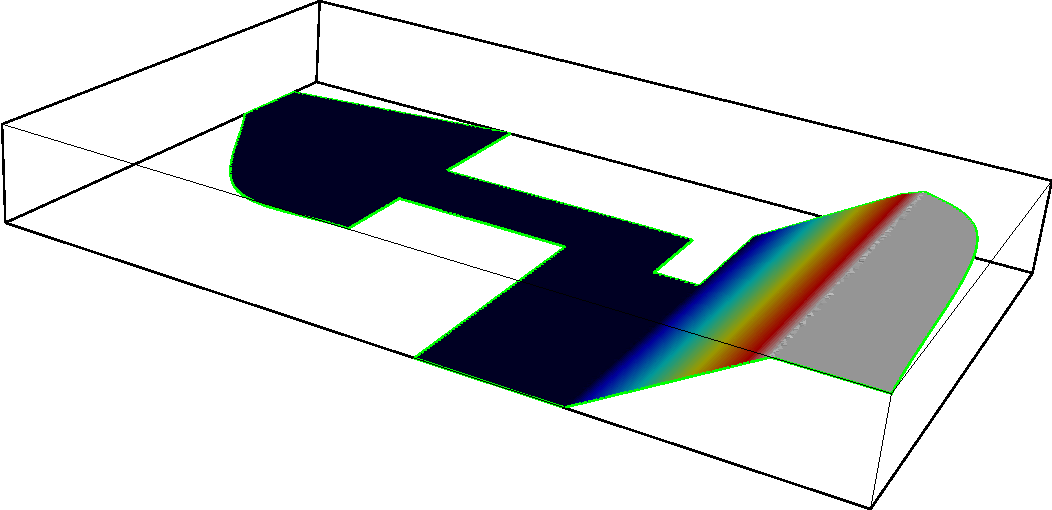
\includegraphics[width=\largefig]{chapters/lopes/pdf/depth.pdf}
  \includegraphics{0001335358/272415_1_en_25_fig21_print.tif}
  \caption{Impermeable bottom $[{\tt Max}=-5.316\,{\tt m},{\tt
      min}=-13.716\,{\tt m}]$.}
  \label{fig:lopes:harbor_depth}\vspace*{8pt}
\end{figure}

\begin{figure}[!t]
%\bwfig
 \narrowfigure
  \centering
  %\fenicsfig{lopes}{sponge_tex}{\largefig}
  \includegraphics{0001335358/272415_1_en_25_fig22_print.eps}
  \caption{Sponge layer (viscosity $\nu(x,y)$) $[{\tt Max} \approx
    0.1\,{\tt m}^2{\tt s}^{-1}, {\tt min}=0 \,{\tt m}^2{\tt s}^{-1}]$.}
  \label{fig:lopes:sponge}\vspace*{8pt}
\end{figure}

\begin{figure}[!t]
%\bwfig
\narrowfigure
  \centering
  %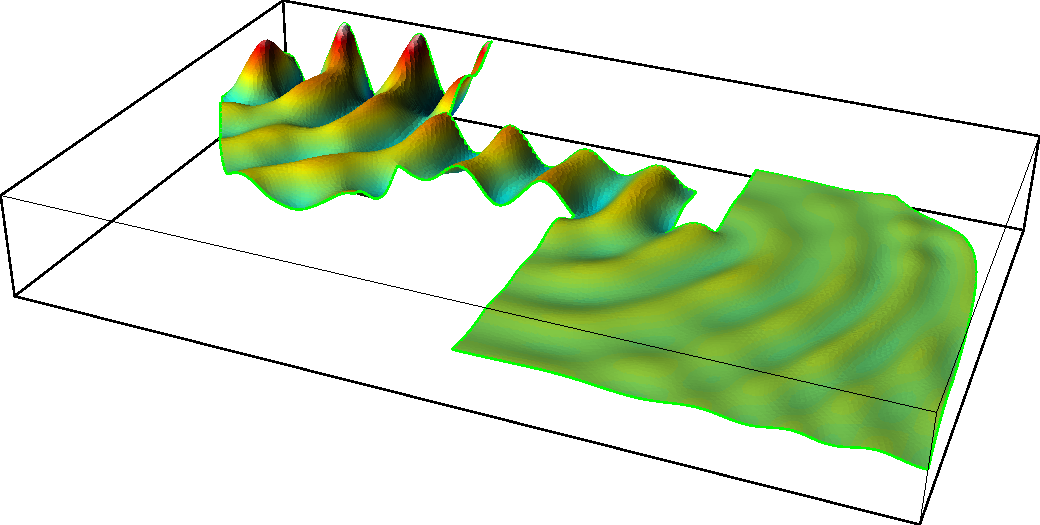
\includegraphics[width=\largefig]{chapters/lopes/pdf/eta.pdf}
  \includegraphics{0001335358/272415_1_en_25_fig23_print.tif}
  \caption{Wave surface elevation $[{\tt Max}\approx 0.63\,{\tt m},
    {\tt min}\approx-0.73\,{\tt m}] $.}\label{fig:lopes:elevation}\vspace*{-6pt}
\end{figure}

\begin{figure}[!t]
%\bwfig
  \centering
  %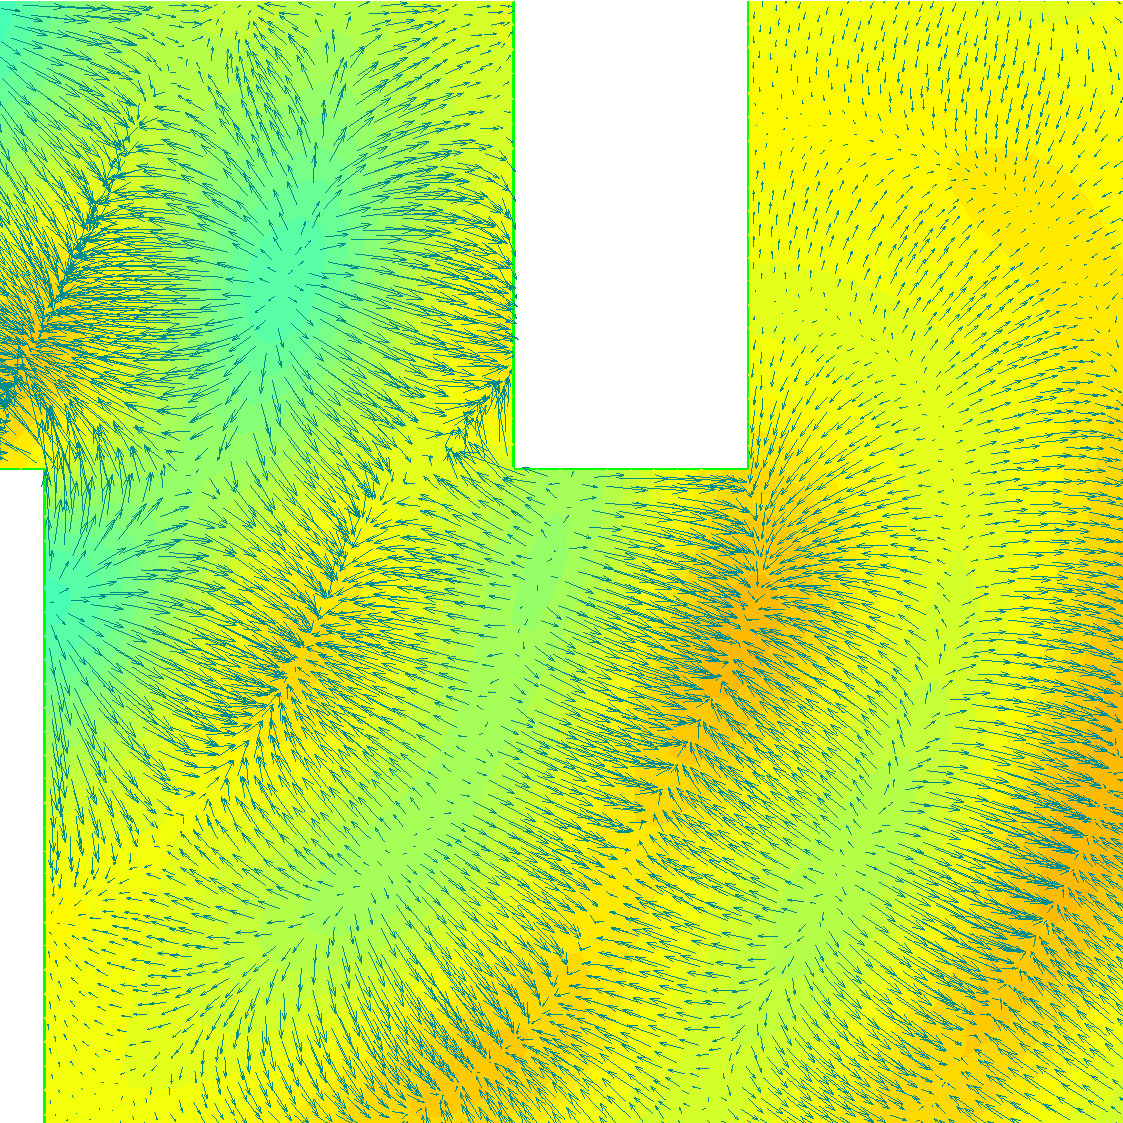
\includegraphics[width=\largefig]{chapters/lopes/pdf/pvel2.pdf}
  \includegraphics{0001335358/272415_1_en_25_fig24_print.tif}
  \caption{Velocity vector field at $z=0$ and potential
    $\phi_0(x,y,t_s)$ near $P_3$. Potential values in $\Omega$: $[{\tt
      Max}\approx 14.2\,{\tt m}^{2}{\tt s}^{-1}, {\tt min}\approx-12.8\,
    {\tt m}^{2}{\tt s}^{-1}]$.}
  \label{fig:lopes:potential1}\vspace*{12pt}
\end{figure}

\begin{figure}[!t]
\centering
\includegraphics{0001335358/272415_1_en_25_fig25_print.eps}
\caption{Wave surface elevation at $P_1$, $P_2$ and $P_3$ $[{\tt
Max}\approx 0.4\, {\tt m}, {\tt min}\approx-0.31\,{\tt
m}]$.}\label{fig:lopes:etap}\vspace*{5pt}
\end{figure}

\begin{figure}[!t]
\centering
\includegraphics{0001335358/272415_1_en_25_fig26_print.eps}
\caption{Water speed at $P_1$, $P_2$ and $P_3$ $[{\tt Max}\approx
0.53\, {\tt m\, s}^{-1}, {\tt min}=0\,{\tt m\, s}^{-1}]$.}
\label{fig:lopes:velp}\vspace*{9pt}
\end{figure}

From these numerical results, we can conclude that the interaction
between incident and reflected waves, near the harbor entrance, can
generate waves with amplitudes that almost take the triple value of
the incident wave amplitude.  We can also observe an analogous
behavior for velocities.  Note that no mechanism for releasing energy
of the reflected waves throughout the incident wave boundary is
considered.

%\enlargethispage{10pt}

\subsection{Object moving on a horizontal bottom}

A wave generated by an object moving on a horizontal bottom with a
constant speed is simulated here.  The declaration of the finite
element discretization of~\eqref{eq:lopes:varform} is that one
described in \hbox{Section}~\ref{sec:lopes:numericalmethods}.

The spatial numerical domain is a rectangular basin of $12.5\times 6\,
{\tt m}^2$ discretized with a symmetric uniform mesh with $2100$
elements.  Full reflective boundary conditions are only considered
here.  The moving bottom $h\, ({\tt m})$ with a constant speed
$S_0=1\, {\tt m\, s}^{-1}$ is defined by
%%
\begin{equation}
  \label{eq:lopes:bottom1}
  h(x,y,t)=0.45-\frac{\Delta h}{(1+\tanh(1))^4}{\bar
    X}(x,t){\bar Y}(y)
\end{equation}

\pagebreak

\noindent with%\vspace*{8pt}
\begin{gather}
{\bar X}(x,t)=(1+\tanh(2(x-x_l(t))))(1-\tanh(2(x-x_r(t)))),\\[12pt]
%\end{equation}
%\begin{equation}
{\bar Y}(y)=(1+\tanh(2y+1)))(1-\tanh(2y-1)),\\[12pt]
%\end{equation}
%%%
%\begin{equation}
\label{eq:lopes:bottom4}
x_l(t)=x_c(t)-\frac{1}{2},\quad
x_r(t)=x_c(t)+\frac{1}{2},\quad x_c(t)=x_0+S_0t,%\vspace*{4pt}
\end{gather}
%%
where $x_0=0\, {\tt m}$ and $\Delta h=0.045\, {\tt
m}$ is the maximum thickness of the slide (see
Figs.~\ref{fig:lopes:objectbottom}--\ref{fig:lopes:objectbottom2}).

\begin{figure}[!t]
%\bwfig
  \centering
  %\includegraphics[width=\largefig]{chapters/lopes/pdf/depth0.pdf}
  \includegraphics{0001335358/272415_1_en_25_fig27_print.eps}
  \caption{The impermeable bottom $-h(x,y,t)$ (m) at the time $t_0=0$
    s. $[{\tt Max}= -0.405\, {\tt m}, {\tt min}=-0.45\,{\tt m}]$}
  \label{fig:lopes:objectbottom}\vspace*{6pt}
%%\vspace*{-6pt}
\end{figure}

\begin{figure}[!t]
%\bwfig
  \centering
  %\includegraphics[width=\largefig]{chapters/lopes/pdf/depth6.pdf}
  \includegraphics{0001335358/272415_1_en_25_fig28_print.eps}
  \caption{The impermeable bottom $-h(x,y,t)$ (m) at the time $t_2=6$
    s. $[{\tt Max}= -0.405\, {\tt m}, {\tt min}=-0.45\,{\tt m}]$}
  \label{fig:lopes:objectbottom2}\vspace*{4pt}
%%\vspace*{-6pt}
\end{figure}

A time step of $\Delta t=0.0005\, {\tt s}$ is considered.  In
Figs. \ref{fig:lopes:objectsurface0}--\ref{fig:lopes:objectsurface3},
we show four snapshots of the wave surface elevation provided by the
extended ZTC model at the time $t_0=1\, {\tt s}$, $t_1=3\, {\tt s}$,
$t_2=4.5\, {\tt s}$ and $t_3=6\, {\tt s}$.  Note that we also use here
the color scale presented in Figure~\ref{fig:lopes:scale}.

\begin{figure}[!t]
%\bwfig
  \centering
  %\includegraphics[width=\largefig]{chapters/lopes/pdf/eta1.pdf}
  \includegraphics{0001335358/272415_1_en_25_fig29_print.eps}
  \caption{The wave surface elevation $\eta$ (m) at the time $t_0=1$
    s. $[{\tt Max}\approx 0.007\, {\tt m}, {\tt min}\approx-0.010\,{\tt m}]$}\label{fig:lopes:objectsurface0}\vspace*{-8pt}
\end{figure}

\begin{figure}[!t]
%\bwfig
  \centering
  %\includegraphics[width=\largefig]{chapters/lopes/pdf/eta3.pdf}
  \includegraphics{0001335358/272415_1_en_25_fig30_print.eps}
  \caption{The wave surface elevation $\eta$ (m) at the time $t_1=3$
    s. $[{\tt Max}\approx 0.004\, {\tt m}, {\tt min}\approx -0.006\, {\tt
        m}]$}
    \label{fig:lopes:objectsurface1}\vspace*{6pt}
\end{figure}

\begin{figure}[!t]
%\bwfig
  \centering
  %\includegraphics[width=\largefig]{chapters/lopes/pdf/eta45.pdf}
  \includegraphics{0001335358/272415_1_en_25_fig31_print.eps}
  \caption{The wave surface elevation $\eta$ (m) at the time
    $t_2=4.5$ s. $[{\tt Max}\approx 0.004\, {\tt m}, {\tt
        min}\approx-0.011\, {\tt m}]$}
    \label{fig:lopes:objectsurface2}
\end{figure}%\clearpage

\begin{figure}[!t]
%\bwfig
  \centering
  %\includegraphics[width=\largefig]{chapters/lopes/pdf/eta6.pdf}
  \includegraphics{0001335358/272415_1_en_25_fig32_print.eps}
  \caption{The wave surface elevation $\eta$ (m) at the time $t_3=6$
    s. $[{\tt Max}\approx 0.004\, {\tt m}, {\tt min}\approx -0.006\,{\tt
        m}]$}
  \label{fig:lopes:objectsurface3}
%\vspace*{6pt}
\end{figure}

We refer that the bottom function given
by~\eqref{eq:lopes:bottom1}--\eqref{eq:lopes:bottom4} is not piecewise
linear. In fact, the spatial derivative functions of any order
obtained from $h$ are nonzero. Although the extended ZTC model is
based on a slowly varying bottom assumption (only $O(h,\nabla h)$
terms are admitted), a good agreement among the solutions presented
here with those provided by other models is achieved (see~\emp{dolfwave/demo/2HD/hLandslide}).  These other models include
$O(h,\nabla h,\nabla^2 h)$ terms (see~\citet{LopesPereiraTrabucho}).

%\enlargethispage{6pt}

\section{Conclusions}

As far as we know, the finite element method is not often applied in
surface water wave models based on the BEP formulation.  In general,
finite difference methods are preferred, since they could be easily
applied to equations containing spatial derivatives with order higher
than 2.  On the other hand, they are not appropriate for the treatment
of complex geometries, like those of harbors, for instance.

In this work, we extend the BEP model of~\citet{ZhaoTengCheng2004} in
order to include dissipative effects, as well as, several types of
wave generation mechanisms, namely, by moving an impermeable bottom or
by the inclusion of a source function.  Moreover, we study the
influence of a dissipative term in the linear dispersive properties,
specifically, in the phase velocity.  We show the existence of some
cutoff values for the wave number such that the short length waves do
not propagate.  From a matrix-based linear stability analysis, we can
also conclude that the ZTC/BEP model is not prone to instabilities of
the type I and II when steep bottom gradients occur or small spatial
grid increments are required.  On the other hand, the standard
potential model with depth averaged velocity potential displays
instabilities for certain combinations of the parameters $l$, $h_m$
and $\Delta x$. The eigenvalue spectra of this model exhibit
interesting structures putting in evidence high growth rates leading
to unstable solutions. Thus, this model should only be applied when
gentle bottom variations occur.  Since we use the same finite element
discretization for both ZTC and standard potential models, some of the
unstable wave modes inherent to the latter one may be intrinsic to the
partial differential equations and not to the numerical schemes.

The extended ZTC equations are used to model four different physical
problems: the evolution of a solitary wave passing through a submerged
bar; the evolution of a Gaussian hump in a square basin; the evolution
of a periodic wave in a harbor and the generation of a wave due to an
object moving on a horizontal bottom.  These equations are discretized
using Lagrange $P_1$ elements and a predictor-corrector scheme with an
initialization provided by an explicit Runge--Kutta method for the
time integration.

In the first physical problem, we can conclude that the numerical
model is also stable when there is an interaction between the incident
and reflected waves over the submerged bar as well as in one of the
domain walls. The shoaling effect over the submerged bar is clearly
observed, both for the incident and reflected waves.  We compare the
solutions of the weakly nonlinear ZTC/BEP and Nwogu/BEV models, for a
spike type submerged bar.  For the employed finite element
discretizations, we observe that the ZTC model is less prone to
instabilities than Nwogu's model.

In the second test, the evolution of a Gaussian hump in a square basin
is simulated.  We obtain a good agreement among the solutions of the
ZTC numerical model and those provided in the FUNWAVE manual.
Moreover, we perform grid refinement tests to ensure convergence and
accuracy.

In the harbor problem, we remark that the interaction between incident
and reflected waves, near the harbor entrance, can generate waves with
amplitudes and velocities that almost take the triple values of those
observed in the incident waves.

In the last numerical example, we refer that the front wave generated
by the moving object travels faster than the object.  In this way, a
subcritical velocity regime associated with the moving object is
observed.  A good agreement among the numerical solutions presented
here with those provided by other models is achieved (see
\emp{dolfwave/demo}).  From these numerical tests we can conclude that
the \fenics packages, namely \dolfin, \ufl and \ffc, are appropriate
to model surface water waves, leading to efficient and robust
algorithms.

Note that strong nonlinear effects, e.g., negative amplitudes
extending below the sea floor, may cause instabilities in a nonlinear
wave model.  These effects will almost certainly be encountered for
instance for a tsunami inundating a shallow sloping beach.  Drying and
wetting schemes for the treatment of these problems are not yet
implemented in DOLFWAVE.  Consequently, this type of instabilities
will most likely show up when running the proposed model with high
amplitude waves and small depth bottoms.

Surface water wave problems are associated with Boussinesq-type
governing equations, which require high order spatial derivatives. A
first approach to a fourth-order spatial derivative model, using a
continuous/discontinuous Galerkin finite element method, can be found
in~\citet{LopesPereiraTrabucho}.

We have been developing DOLFWAVE which is a \fenics based application
for surface water wave models. This package already includes some
models with equations containing spatial derivatives of order~$4$.
The current state of the work, along with several numerical
simulations, can be found at \url{http://ptmat.fc.ul.pt/~ndl} and
\url{https://launchpad.net/dolfwave}.

\endgroup




%%%%\begin{figure}
%%%%\includegraphics{0001335358/272415_1_en_25_fig25_print.eps}
%%%%\caption{}
%%%%\end{figure}
%%%%\begin{figure}
%%%%\includegraphics{0001335358/272415_1_en_25_fig26_print.eps}
%%%%\caption{}
%%%%\end{figure}
%%%%\begin{figure}
%%%%\includegraphics{0001335358/272415_1_en_25_fig27_print.eps}
%%%%\caption{}
%%%%\end{figure}
%%%%\begin{figure}
%%%%\includegraphics{0001335358/272415_1_en_25_fig28_print.eps}
%%%%\caption{}
%%%%\end{figure}
%%%%\begin{figure}
%%%%\includegraphics{0001335358/272415_1_en_25_fig29_print.eps}
%%%%\caption{}
%%%%\end{figure}
%%%%\begin{figure}
%%%%\includegraphics{0001335358/272415_1_en_25_fig30_print.eps}
%%%%\caption{}
%%%%\end{figure}
%%%%\begin{figure}
%%%%\includegraphics{0001335358/272415_1_en_25_fig31_print.eps}
%%%%\caption{}
%%%%\end{figure}
%%%%\begin{figure}
%%%%\includegraphics{0001335358/272415_1_en_25_fig32_print.eps}
%%%%\caption{}
%%%%\end{figure}
%%%%\begin{figure}
%%%%\includegraphics{0001335358/272415_1_en_25_fig24_print.tif}
%%%%\caption{}
%%%%\end{figure}
%%%%\begin{figure}
%%%%\includegraphics{0001335358/272415_1_en_25_fig23_print.tif}
%%%%\caption{}
%%%%\end{figure}
%%%%\begin{figure}
%%%%\includegraphics{0001335358/272415_1_en_25_fig22_print.eps}
%%%%\caption{}
%%%%\end{figure}
%%%%\begin{figure}
%%%%\includegraphics{0001335358/272415_1_en_25_fig21_print.tif}
%%%%\caption{}
%%%%\end{figure}
%%%%\begin{figure}
%%%%\includegraphics{0001335358/272415_1_en_25_fig20_print.eps}
%%%%\caption{}
%%%%\end{figure}
%%%%\begin{figure}
%%%%\includegraphics{0001335358/272415_1_en_25_fig19_print.eps}
%%%%\caption{}
%%%%\end{figure}
%%%%\begin{figure}
%%%%\includegraphics{0001335358/272415_1_en_25_fig18_print.eps}
%%%%\caption{}
%%%%\end{figure}
%%%%\begin{figure}
%%%%\includegraphics{0001335358/272415_1_en_25_fig17_print.tif}
%%%%\caption{}
%%%%\end{figure}
%%%%\begin{figure}
%%%%\includegraphics{0001335358/272415_1_en_25_fig16_print.eps}
%%%%\caption{}
%%%%\end{figure}
%%%%\begin{figure}
%%%%\includegraphics{0001335358/272415_1_en_25_fig15_print.eps}
%%%%\caption{}
%%%%\end{figure}
%%%%\begin{figure}
%%%%\includegraphics{0001335358/272415_1_en_25_fig14_print.eps}
%%%%\caption{}
%%%%\end{figure}
%%%%\begin{figure}
%%%%\includegraphics{0001335358/272415_1_en_25_fig13_print.eps}
%%%%\caption{}
%%%%\end{figure}
%%%%\begin{figure}
%%%%\includegraphics{0001335358/272415_1_en_25_fig12_print.eps}
%%%%\caption{}
%%%%\end{figure}
%%%%\begin{figure}
%%%%\includegraphics{0001335358/272415_1_en_25_fig11_print.eps}
%%%%\caption{}
%%%%\end{figure}
%%%%\begin{figure}
%%%%\includegraphics{0001335358/272415_1_en_25_fig10_print.tif}
%%%%\caption{}
%%%%\end{figure}
%%%%\begin{figure}
%%%%\includegraphics{0001335358/272415_1_en_25_fig9_print.tif}
%%%%\caption{}
%%%%\end{figure}
%%%%\begin{figure}
%%%%\includegraphics{0001335358/272415_1_en_25_fig8_print.tif}
%%%%\caption{}
%%%%\end{figure}
%%%%\begin{figure}
%%%%\includegraphics{0001335358/272415_1_en_25_fig7_print.tif}
%%%%\caption{}
%%%%\end{figure}
%%%%\begin{figure}
%%%%\includegraphics{0001335358/272415_1_en_25_fig6_print.tif}
%%%%\caption{}
%%%%\end{figure}
%%%%\begin{figure}
%%%%\includegraphics{0001335358/272415_1_en_25_fig5_print.tif}
%%%%\caption{}
%%%%\end{figure}
%%%%\begin{figure}
%%%%\includegraphics{0001335358/272415_1_en_25_fig4_print.eps}
%%%%\caption{}
%%%%\end{figure}
%%%%\begin{figure}
%%%%\includegraphics{0001335358/272415_1_en_25_fig3_print.eps}
%%%%\caption{}
%%%%\end{figure}
%%%%\begin{figure}
%%%%\includegraphics{0001335358/272415_1_en_25_fig2_print.eps}
%%%%\caption{}
%%%%\end{figure}
%%%%\begin{figure}
%%%%\includegraphics{0001335358/272415_1_en_25_fig1_print.tif}
%%%%\caption{}
%%%%\end{figure} 